% Slides: project status, current results and the training / test campaigns still to run.
% Build: make status-pdf (pdflatex). Results come from ../article/generated.tex, regenerated by
% `make article`: never type a result by hand here. Durations and run lists are plans, copied
% from docs/tasks/long-runs.md (state 2026-10-20) and cited on each slide.
\documentclass[aspectratio=169,11pt]{beamer}
\usetheme[progressbar=frametitle,numbering=fraction]{metropolis}
\usepackage[utf8]{inputenc}
\usepackage[T1]{fontenc}
\usepackage{lmodern}
\DeclareUnicodeCharacter{2212}{\ensuremath{-}}
\usepackage{amsmath,amssymb}
\usepackage{graphicx}
\usepackage{booktabs,tabularx,array}
\usepackage{xcolor}
\usepackage{tikz}
\usetikzlibrary{positioning,arrows.meta}

% Generated by `python -m tools.article render` (make article): do not edit by hand.
% Numbers: docs/article/chiffres.json; figures: tools/figures; status: docs/tasks/README.md.
\newcommand\artget[2]{\ifcsname art#1:#2\endcsname\csname art#1:#2\endcsname
  \else\PackageError{article}{unknown #1 key '#2' (make article)}{}\fi}
\newcommand\chiffre[1]{\artget{n}{#1}}
\newcommand\articletable[1]{\artget{table}{#1}}
\newcommand\articlefig[1]{\artget{fig}{#1}}

% ---- numbers
\expandafter\def\csname artn:balayage.crowdhuman.meilleur.map\endcsname{%
35.87\textsuperscript{tier R}}  % tier-R, docs/tasks/resultats-balayages.md
\expandafter\def\csname artn:balayage.exdark.meilleur.map\endcsname{%
13.29\textsuperscript{tier R}}  % tier-R, docs/tasks/resultats-balayages.md
\expandafter\def\csname artn:balayage.flir.meilleur.map\endcsname{%
0.70\textsuperscript{tier R}}  % tier-R, docs/tasks/resultats-balayages.md
\expandafter\def\csname artn:balayage.kitti.meilleur.map\endcsname{%
2.38\textsuperscript{tier R}}  % tier-R, docs/tasks/resultats-balayages.md
\expandafter\def\csname artn:balayage.visdrone.meilleur.map\endcsname{%
2.24\textsuperscript{tier R}}  % tier-R, docs/tasks/resultats-balayages.md
\expandafter\def\csname artn:balayage.voc.meilleur.map\endcsname{%
36.27\textsuperscript{tier R}}  % tier-R, docs/tasks/resultats-balayages.md
\expandafter\def\csname artn:map.formats.admm\endcsname{%
43.07}  % measured, results/req_yolo.md
\expandafter\def\csname artn:map.formats.hwpp\endcsname{%
55.56}  % measured, results/postproc_hw.md
\expandafter\def\csname artn:map.formats.mixed6\endcsname{%
52.46}  % measured, results/req_yolo.md
\expandafter\def\csname artn:map.formats.uniform6\endcsname{%
54.35}  % measured, results/req_yolo.md
\expandafter\def\csname artn:map.formats.w4a4.ptq\endcsname{%
17.06}  % measured, results/quant_4bits.md
\expandafter\def\csname artn:map.formats.w4a4.qat\endcsname{%
36.38}  % measured, results/quant_4bits.md
\expandafter\def\csname artn:map.voc.csim\endcsname{%
55.66\textsuperscript{C-sim}}  % csim, results/map_stades.md
\expandafter\def\csname artn:map.voc.darknet\endcsname{%
57.1\textsuperscript{pub.}}  % published, results/map_float.md
\expandafter\def\csname artn:map.voc.drop\endcsname{%
−0.64}  % measured, results/map_stades.md
\expandafter\def\csname artn:map.voc.float\endcsname{%
56.30}  % measured, results/map_stades.md
\expandafter\def\csname artn:map.voc.identical\endcsname{%
4,952\textsuperscript{C-sim}}  % csim, results/map_stades.md
\expandafter\def\csname artn:map.voc.images\endcsname{%
4,952}  % measured, results/map_stades.md
\expandafter\def\csname artn:map.voc.int8\endcsname{%
55.66}  % measured, results/map_stades.md
\expandafter\def\csname artn:model.v2.gmacs\endcsname{%
3.49}  % measured, python/yolo/models/specs.py
\expandafter\def\csname artn:model.v2.mparams\endcsname{%
15.86}  % measured, python/yolo/models/specs.py
\expandafter\def\csname artn:model.v3.gmacs\endcsname{%
2.74}  % measured, python/yolo/models/specs.py
\expandafter\def\csname artn:model.v3.mparams\endcsname{%
8.71}  % measured, python/yolo/models/specs.py
\expandafter\def\csname artn:perf.kv260.bound.ms\endcsname{%
31.6\textsuperscript{proj.}}  % projection, results/rapport.md
\expandafter\def\csname artn:perf.kv260.m6.ms\endcsname{%
206.5\textsuperscript{proj.}}  % projection, results/rapport.md
\expandafter\def\csname artn:perf.kv260.roofline.ms\endcsname{%
31.9\textsuperscript{proj.}}  % projection, results/rapport.md
\expandafter\def\csname artn:perf.kv260.v2.eff\endcsname{%
61.0\textsuperscript{proj.}}  % projection, results/mesures.md
\expandafter\def\csname artn:perf.kv260.v2.fps\endcsname{%
26.9\textsuperscript{proj.}}  % projection, results/mesures.md
\expandafter\def\csname artn:perf.kv260.v2.gops\endcsname{%
187.3\textsuperscript{proj.}}  % projection, results/mesures.md
\expandafter\def\csname artn:perf.kv260.v2.ms\endcsname{%
37.2\textsuperscript{proj.}}  % projection, results/mesures.md
\expandafter\def\csname artn:perf.kv260.v3.ms\endcsname{%
36.1\textsuperscript{proj.}}  % projection, results/mesures.md
\expandafter\def\csname artn:quant.sensitive.gap\endcsname{%
−0.61\textsuperscript{tier R}}  % tier-R, results/map_int8.md
\expandafter\def\csname artn:quant.sensitive.layer\endcsname{%
L10\textsuperscript{tier R}}  % tier-R, results/map_int8.md
\expandafter\def\csname artn:stream.w4.fps\endcsname{%
64.2\textsuperscript{est.}}  % estimate, results/streaming.md
\expandafter\def\csname artn:stream.w8.dsp\endcsname{%
968\textsuperscript{est.}}  % estimate, results/streaming.md
\expandafter\def\csname artn:stream.w8.fps\endcsname{%
32.1\textsuperscript{est.}}  % estimate, results/streaming.md
\expandafter\def\csname artn:stream.w8.latency\endcsname{%
85.2\textsuperscript{est.}}  % estimate, results/streaming.md
\expandafter\def\csname artn:verif.dumps\endcsname{%
6}  % measured, Makefile (DUMP_IMAGES × QNETS)
\expandafter\def\csname artn:verif.hwpp.cases\endcsname{%
1,014\textsuperscript{C-sim}}  % csim, results/postproc_hw.md
% ---- tables
\expandafter\def\csname arttable:balayages.meilleurs\endcsname{%
\setlength{\tabcolsep}{4pt}
\begin{tabularx}{\linewidth}{@{}>{\raggedright\arraybackslash}Xr>{\raggedright\arraybackslash}Xr>{\raggedright\arraybackslash}X>{\raggedright\arraybackslash}Xr>{\raggedright\arraybackslash}X@{}}
\toprule
\textbf{Dataset} & \textbf{\begin{tabular}[b]{@{}r@{}}Training\\images\end{tabular}} & \textbf{Best run} & \textbf{Batch} & \textbf{Training subset} & \textbf{Metric} & \textbf{\begin{tabular}[b]{@{}r@{}}Score (50\\images)\end{tabular}} & \textbf{Status} \\
\midrule
VOC & 16,551 & \texttt{b32-sall} & 32 & all & mAP, 11 points & 36.27 & tier-R \\
VisDrone & 6,471 & \texttt{b32-sall} & 32 & all & mAP, 11 points & 2.24 & tier-R \\
KITTI & 5,985 & \texttt{b32-sall} & 32 & all & mAP, 11 points & 2.38 & tier-R \\
FLIR & 10,742 & \texttt{b8-sall} & 8 & all & AP@[.5:.95] (COCO) & 0.70 & tier-R \\
ExDark & 3,000 & \texttt{b32-sall} & 32 & all & mAP, 11 points & 13.29 & tier-R \\
CrowdHuman & 15,000 & \texttt{b16-sall} & 16 & all & mAP, 11 points & 35.87 & tier-R \\
\bottomrule
\end{tabularx}}
\expandafter\def\csname arttable:benchmarks\endcsname{%
\setlength{\tabcolsep}{4pt}
\begin{tabularx}{\linewidth}{@{}>{\raggedright\arraybackslash}X>{\raggedright\arraybackslash}X>{\raggedright\arraybackslash}X>{\raggedright\arraybackslash}X>{\raggedright\arraybackslash}X>{\raggedright\arraybackslash}X>{\raggedright\arraybackslash}X>{\raggedright\arraybackslash}X>{\raggedright\arraybackslash}X@{}}
\toprule
\textbf{Work} & \textbf{Model} & \textbf{FPGA} & \textbf{Format} & \textbf{img/s} & \textbf{ms} & \textbf{GOPS} & \textbf{W} & \textbf{Status} \\
\midrule
2023-zhai & YOLOv3-tiny pruned, 1 module & Zynq XC7Z035 & INT16 & 91.65 & — & 67.91 & 12.51 & published \\
2023-zhai & YOLOv3-tiny pruned, 2 modules & Zynq XC7Z035 & INT16 & 168.72 & — & 124.01 & 15.18 & published \\
2024-zhang & YOLOv2-Tiny 416, batch 1 & Kintex-7 325T & INT8 & — & 14.49 & 406 & 12.3 & published \\
2024-zhang & YOLOv3-Tiny 416, batch 1 & Kintex-7 325T & INT8 & — & 15.2 & 401 & 12.3 & published \\
2023-montgomerie-corcoran & YOLOv3-Tiny 416 & VCU110 & W8A16 & — & — & 418.9 & 15.4 & published \\
2019-ding & Tiny-YOLOv2, ADMM heterogeneous & Virtex-7 690T & FFT + powers of 2 & 314.2 & — & — & 21 & published \\
2026-fata & YOLOv3-tiny pruned at 70 \% (DPU Vitis AI) & Kria KV260 (DPU) & INT8 QAT & 24.3 & — & 60.18 & 2.13 & published \\
2025-kim & YOLOv2 full (prototype) & Zybo Z7-20 & INT16 & 0.083 & 12,000 & — & — & published \\
this work (C-sim projection) & Tiny-YOLOv2 VOC 416 & Kria KV260 (XCK26) & INT8 (W8A8, per channel) & 26.87 & 37.2 & 187.3 & — & projection \\
this work (C-sim projection) & Tiny-YOLOv3 COCO 416 & Kria KV260 (XCK26) & INT8 (W8A8, per channel) & 27.72 & 36.1 & 154.3 & — & projection \\
\bottomrule
\end{tabularx}}
\expandafter\def\csname arttable:map.formats\endcsname{%
\setlength{\tabcolsep}{4pt}
\begin{tabularx}{\linewidth}{@{}>{\raggedright\arraybackslash}X>{\raggedright\arraybackslash}Xrr@{}}
\toprule
\textbf{Weights / activations} & \textbf{Method} & \textbf{mAP} & \textbf{\begin{tabular}[b]{@{}r@{}}Gap to\\INT8\end{tabular}} \\
\midrule
INT8 per channel (reference) & PTQ & 55.66 & — \\
uniform6 (±31) & PTQ & 54.35 & −1.31 \\
mixed6 (powers of 2) & PTQ, direct projection & 52.46 & −3.20 \\
mixed6 & ADMM, 600 iterations, then projection & 43.07 & −12.59 \\
w4a4 & PTQ (power-of-2 steps) & 17.06 & −38.60 \\
w4a4 & QAT, 600 iterations & 36.38 & −19.28 \\
INT8 + hardware post-processing & unsorted NMS, Q4 boxes & 55.56 & −0.10 \\
\bottomrule
\end{tabularx}}
\expandafter\def\csname arttable:map.stades\endcsname{%
\setlength{\tabcolsep}{4pt}
\begin{tabularx}{\linewidth}{@{}>{\raggedright\arraybackslash}Xr>{\raggedright\arraybackslash}X>{\raggedright\arraybackslash}X@{}}
\toprule
\textbf{Stage} & \textbf{mAP} & \textbf{Equality with the integer model} & \textbf{Status} \\
\midrule
Float (fused BN, NumPy float32) & 56.30 & — & measured \\
Integer, Python (\texttt{IntNetwork}, bit-exact) & 55.66 & reference & measured \\
FPGA, C-sim (ARM driver, sim backend, PC) & 55.66 & 4,952 / 4,952 identical images & csim \\
FPGA, KV260 (uio backend) & — & to be measured & — \\
\bottomrule
\end{tabularx}}
\expandafter\def\csname arttable:map.voc.float.table\endcsname{%
\setlength{\tabcolsep}{4pt}
\begin{tabularx}{\linewidth}{@{}>{\raggedright\arraybackslash}X>{\raggedright\arraybackslash}Xr@{}}
\toprule
\textbf{Preprocessing} & \textbf{Interpolation} & \textbf{mAP} \\
\midrule
direct resize (\texttt{stretch}) & Pillow bilinear & 56.30 \\
direct resize (\texttt{stretch}) & Darknet (\texttt{resize\_image}) & 56.32 \\
letterbox & Pillow bilinear & 54.18 \\
letterbox & Darknet (\texttt{resize\_image}) & 53.98 \\
\bottomrule
\end{tabularx}}
\expandafter\def\csname arttable:map.voc.int8.table\endcsname{%
\setlength{\tabcolsep}{4pt}
\begin{tabularx}{\linewidth}{@{}>{\raggedright\arraybackslash}Xrrr@{}}
\toprule
\textbf{Preprocessing} & \textbf{\begin{tabular}[b]{@{}r@{}}Float\\(fused BN)\end{tabular}} & \textbf{\begin{tabular}[b]{@{}r@{}}Integer\\INT8\end{tabular}} & \textbf{Gap} \\
\midrule
stretch (\texttt{make eval-float}) & 56.30 & 55.66 & −0.64 \\
letterbox (the training one) & 54.18 & 53.68 & −0.50 \\
\bottomrule
\end{tabularx}}
\expandafter\def\csname arttable:perf.cascade\endcsname{%
\setlength{\tabcolsep}{4pt}
\begin{tabularx}{\linewidth}{@{}>{\raggedright\arraybackslash}Xrrrrr@{}}
\toprule
\textbf{Kernel configuration (Tiny-YOLOv2)} & \textbf{Mcycles} & \textbf{ms} & \textbf{img/s} & \textbf{GOPS} & \textbf{\begin{tabular}[b]{@{}r@{}}MAC efficiency\\(\%)\end{tabular}} \\
\midrule
M6: ports 8 bits & 41.30 & 206.5 & 4.8 & 33.8 & 11.0 \\
valid channels only (trim) & 32.67 & 163.3 & 6.1 & 42.7 & 13.9 \\
ports 64 bits & 12.27 & 61.3 & 16.3 & 113.6 & 37.0 \\
ports 128 bits + trim & 12.13 & 60.6 & 16.5 & 115.0 & 37.4 \\
ports 64 bits + trim + requantization ×8 (+28 DSP) & 9.29 & 46.4 & 21.5 & 150.1 & 48.9 \\
... + L00 folding & 8.38 & 41.9 & 23.9 & 166.4 & 54.2 \\
... + 14×14 tiles for pooled convs (M10 kernel) & 7.44 & 37.2 & 26.9 & 187.3 & 61.0 \\
compute bound of M6 (free loads) & 8.23 & 41.1 & 24.3 & 169.5 & 55.2 \\
compute bound of the M10 kernel & 6.32 & 31.6 & 31.7 & 220.7 & 71.8 \\
KV260 roofline point (roofline.md) & — & 31.9 & 31.3 & 218.5 & — \\
ideal (MACs / 768, efficiency 100 \%) & 4.54 & 22.7 & 44.1 & 307.2 & 100.0 \\
\bottomrule
\end{tabularx}
\par\smallskip{\footnotesize\emph{Status of every number of this table: projection.}}}
\expandafter\def\csname arttable:perf.kv260\endcsname{%
\setlength{\tabcolsep}{4pt}
\begin{tabularx}{\linewidth}{@{}>{\raggedright\arraybackslash}Xrrrrrr>{\raggedright\arraybackslash}X@{}}
\toprule
\textbf{Network} & \textbf{GMAC} & \textbf{Mcycles} & \textbf{ms} & \textbf{img/s} & \textbf{GOPS} & \textbf{\begin{tabular}[b]{@{}r@{}}MAC efficiency\\(\%)\end{tabular}} & \textbf{Status} \\
\midrule
\texttt{tiny-yolov2-voc} & 3.486 & 7.44 & 37.2 & 26.9 & 187.3 & 61.0 & projection \\
\texttt{tiny-yolov3-coco} & 2.782 & 7.21 & 36.1 & 27.7 & 154.3 & 50.2 & projection \\
\bottomrule
\end{tabularx}}
% ---- figures cited by article.tex
\expandafter\def\csname artfig:etat_art\endcsname{%
\begin{figure}[htbp]
\centering
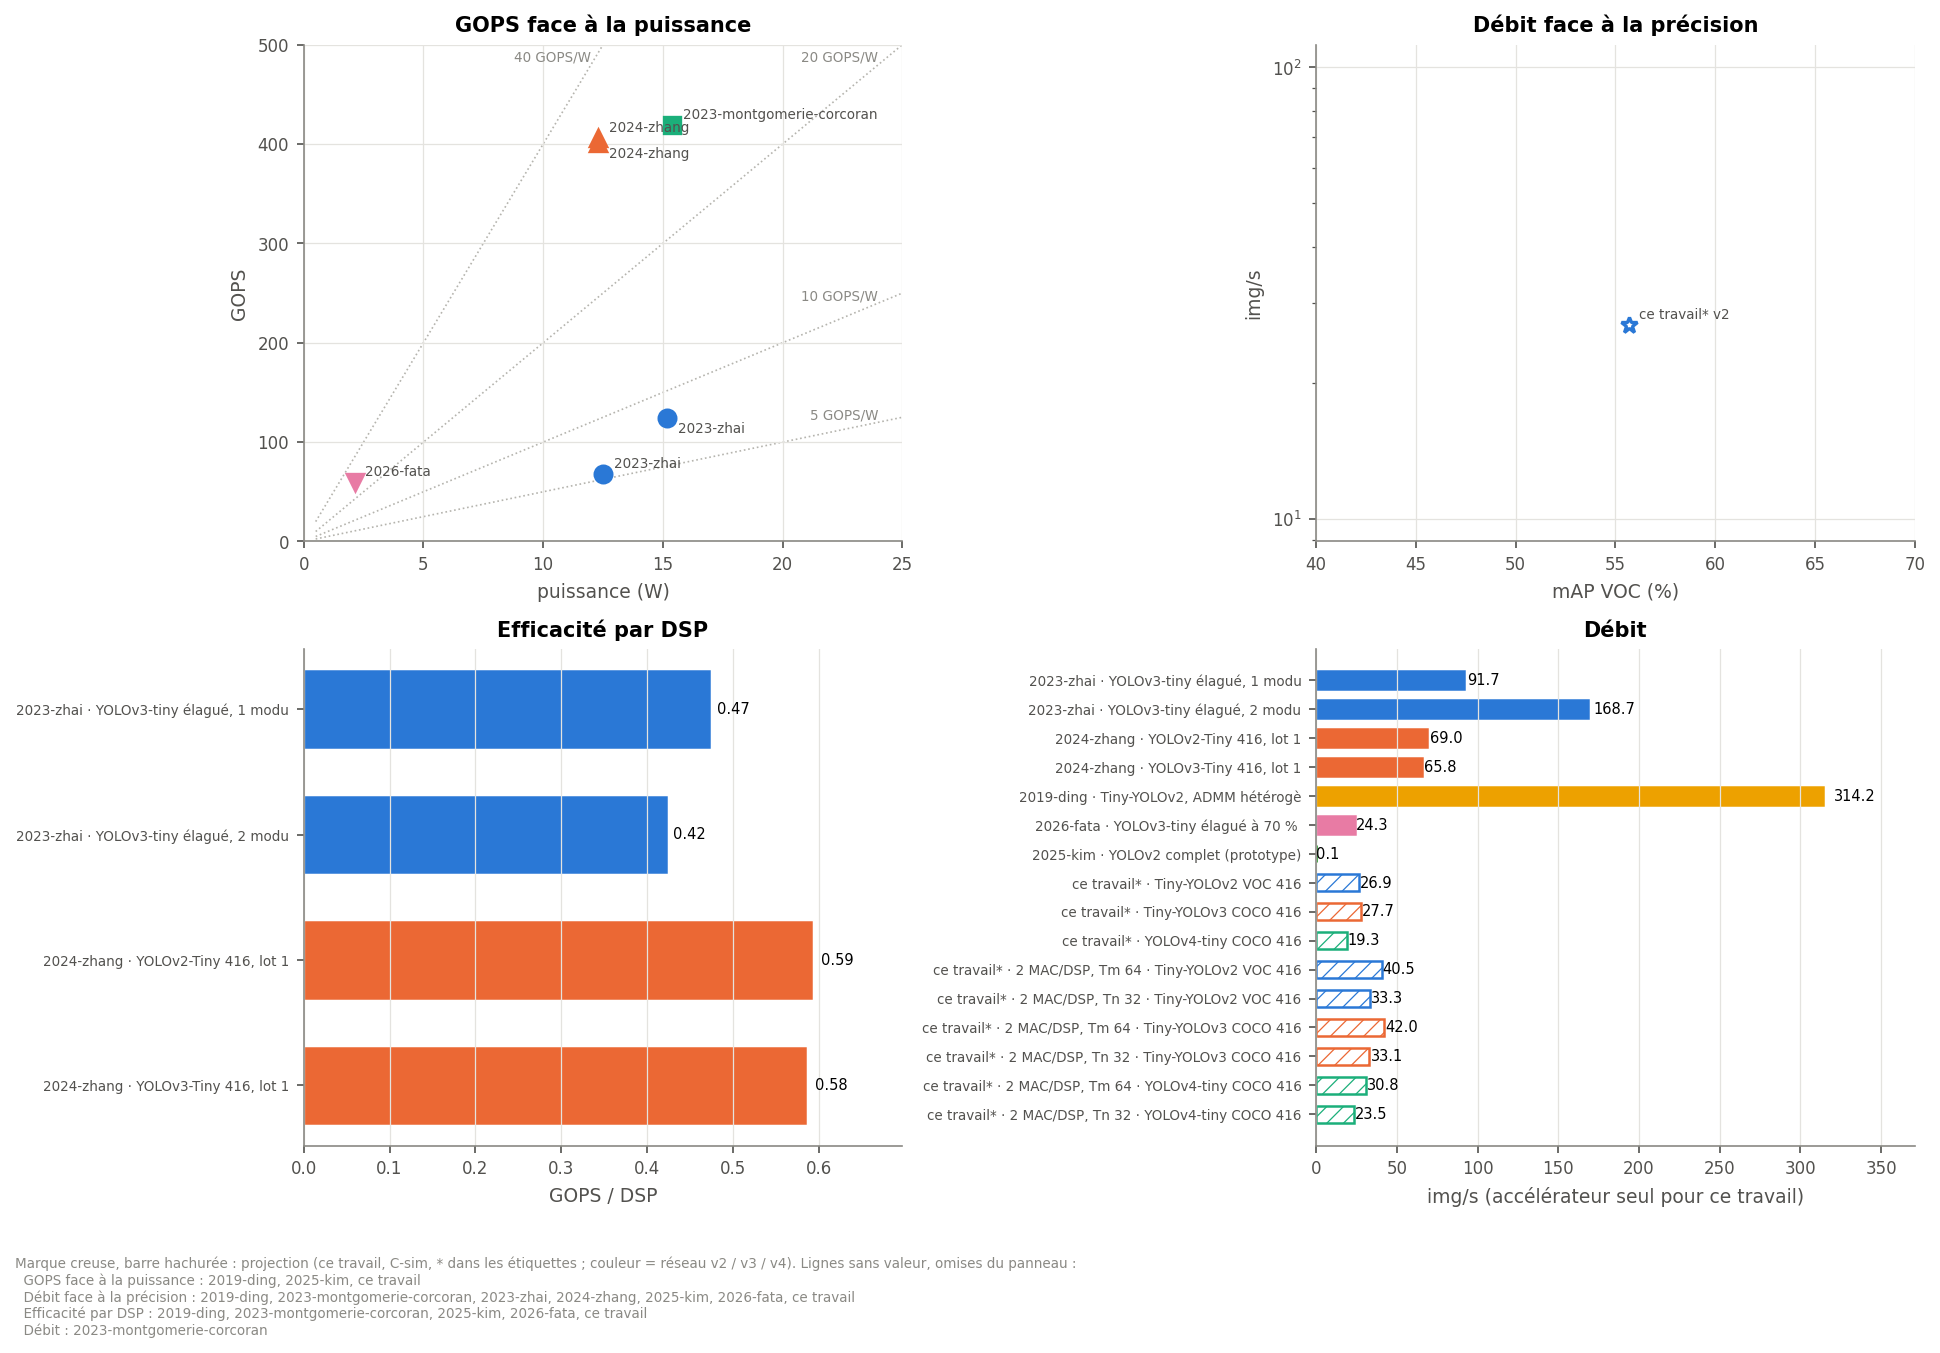
\includegraphics[width=\linewidth,height=0.42\textheight,keepaspectratio]{../../results/figures/resultats/etat_art.png}
\caption{Comparaison aux accélérateurs publiés : GOPS et puissance, débit et mAP, GOPS par DSP (marque creuse : projection de ce travail). (\texttt{etat\_art})}
\label{fig:etat_art}
% python -m tools.figures etat_art
\end{figure}}
\expandafter\def\csname artfig:graphe/graphe_tiny-yolov2-voc\endcsname{%
\begin{figure}[htbp]
\centering
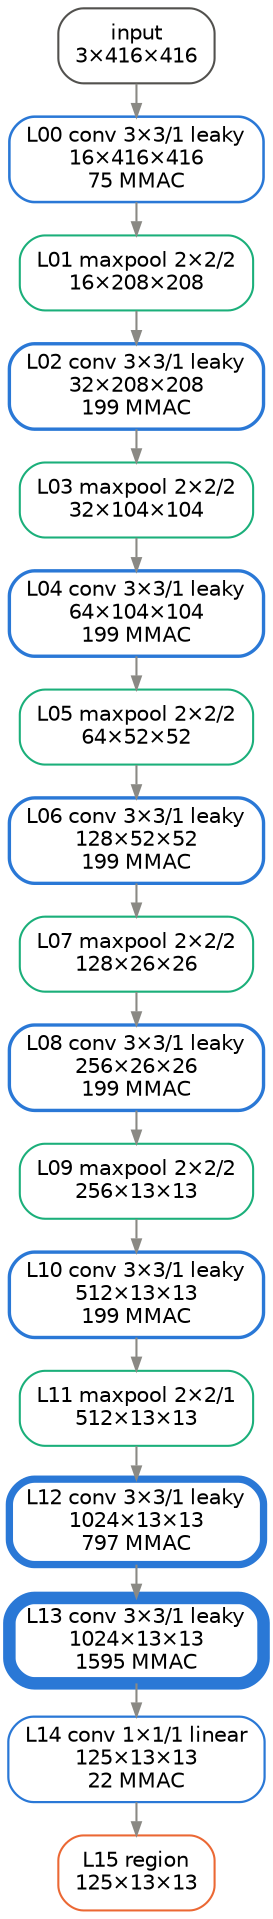
\includegraphics[width=\linewidth,height=0.42\textheight,keepaspectratio]{../../results/figures/modeles/graphe_tiny-yolov2-voc.png}
\caption{Graphe couche par couche (type, noyau et stride, forme de sortie C×H×W ; bord épais = beaucoup de MACs). (\texttt{graphe})}
\label{fig:graphe/graphe_tiny-yolov2-voc}
% python -m tools.figures graphe
\end{figure}}
\expandafter\def\csname artfig:fiche/fiche_tiny-yolov2-voc\endcsname{%
\begin{figure}[htbp]
\centering
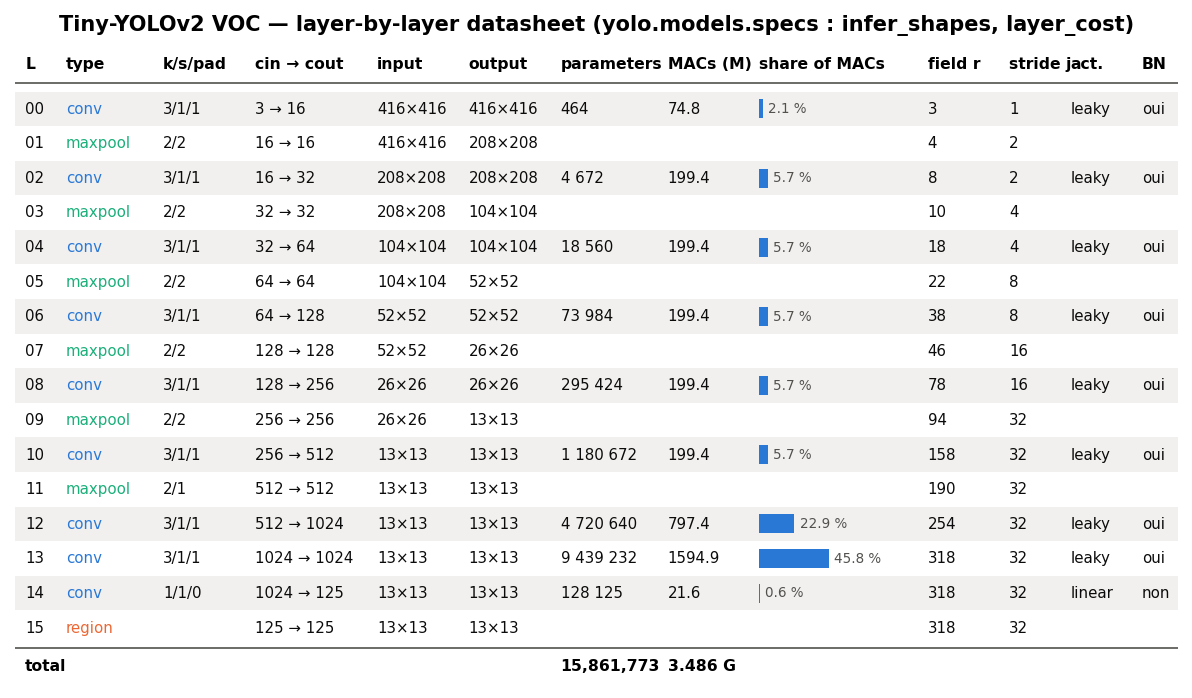
\includegraphics[width=\linewidth,height=0.42\textheight,keepaspectratio]{../../results/figures/reseaux/fiche_tiny-yolov2-voc.png}
\caption{Fiche couche par couche : type, noyau, formes, paramètres, MACs et leur part, champ réceptif et pas cumulé (CSV à côté de l'image). (\texttt{fiche})}
\label{fig:fiche/fiche_tiny-yolov2-voc}
% python -m tools.figures fiche
\end{figure}}
\expandafter\def\csname artfig:convolution\endcsname{%
\begin{figure}[htbp]
\centering
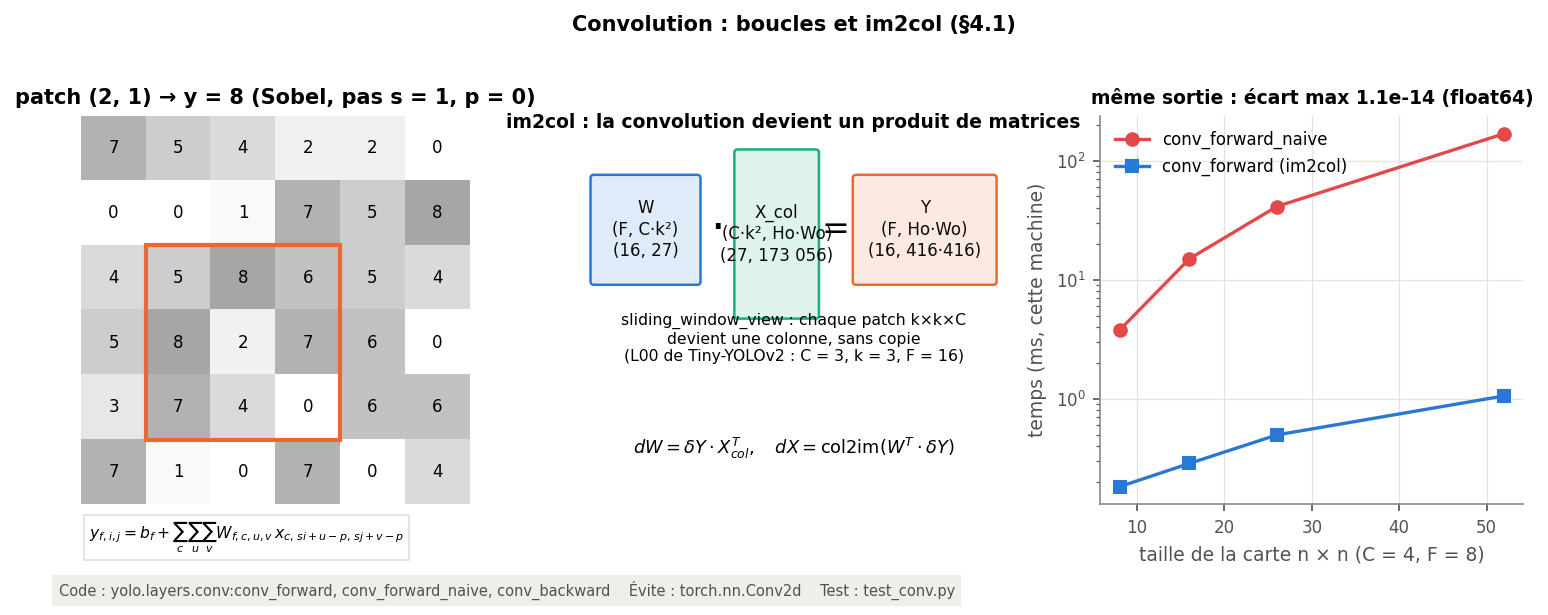
\includegraphics[width=\linewidth,height=0.42\textheight,keepaspectratio]{../../results/figures/maths/convolution.png}
\caption{Convolution : la formule sur un patch, le dépliage im2col en produit de matrices, et le temps des boucles face à im2col. (\texttt{convolution})}
\label{fig:convolution}
% python -m tools.figures convolution
\end{figure}}
\expandafter\def\csname artfig:retropropagation\endcsname{%
\begin{figure}[htbp]
\centering
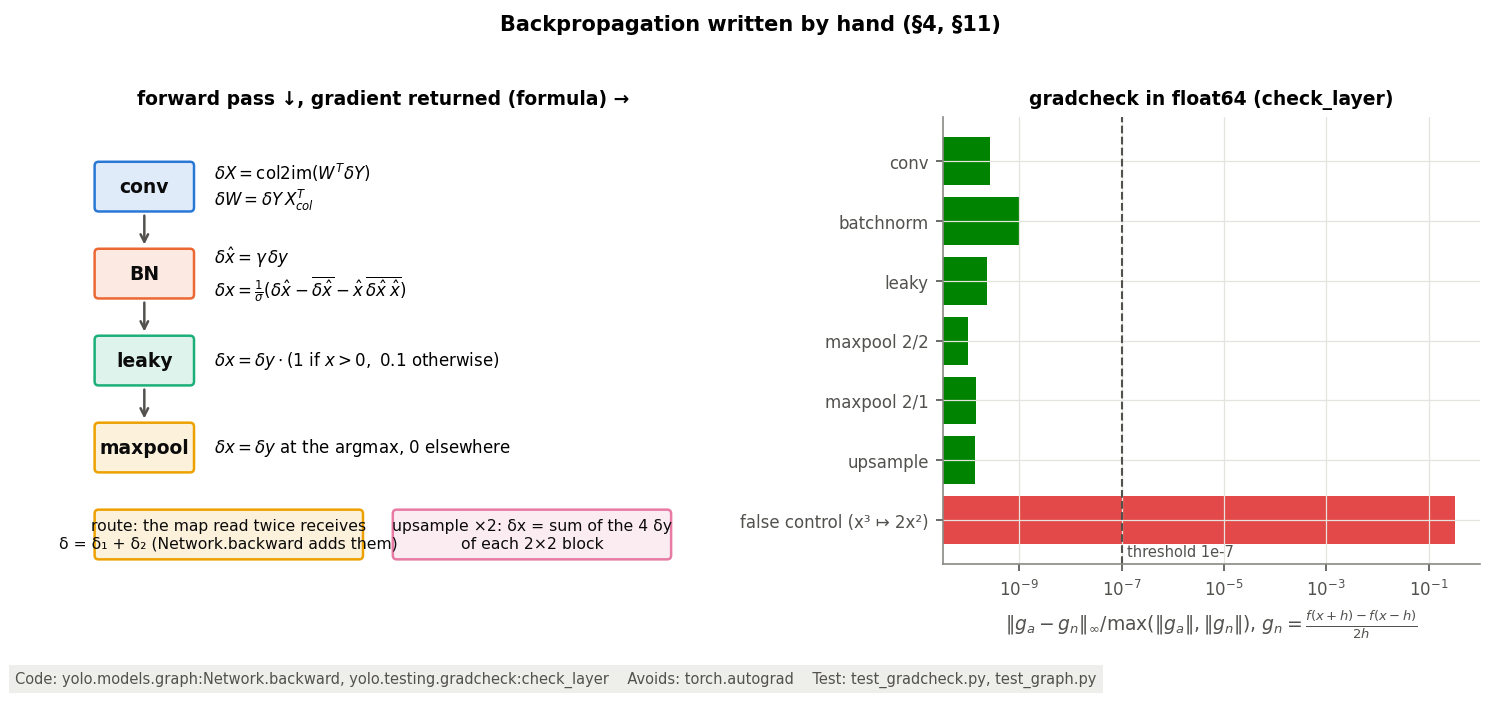
\includegraphics[width=\linewidth,height=0.42\textheight,keepaspectratio]{../../results/figures/maths/retropropagation.png}
\caption{Rétropropagation écrite à la main : formule du gradient renvoyé par chaque couche, puis l'erreur du gradcheck par couche face au seuil 1e-7. (\texttt{retropropagation})}
\label{fig:retropropagation}
% python -m tools.figures retropropagation
\end{figure}}
\expandafter\def\csname artfig:perte\endcsname{%
\begin{figure}[htbp]
\centering
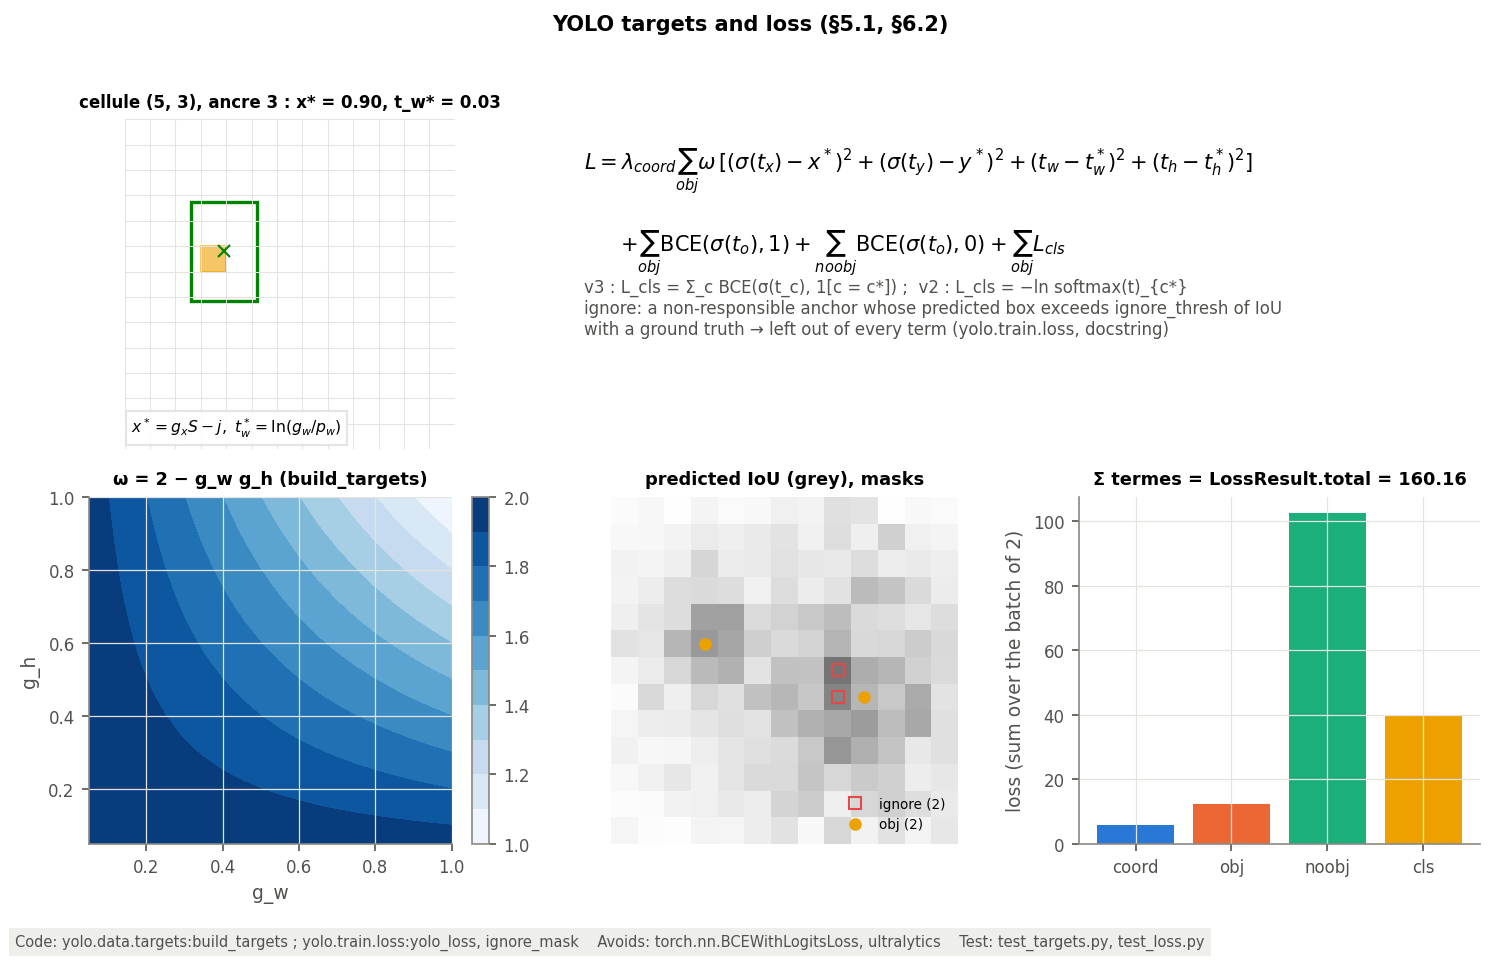
\includegraphics[width=\linewidth,height=0.42\textheight,keepaspectratio]{../../results/figures/maths/perte.png}
\caption{Cibles et perte YOLO : encodage d'une vérité, la perte terme par terme, le poids $\omega$ = 2 − g\_w g\_h, le masque ignore et la part de chaque terme sur un lot. (\texttt{perte})}
\label{fig:perte}
% python -m tools.figures perte
\end{figure}}
\expandafter\def\csname artfig:pr/pr_variantes\endcsname{%
\begin{figure}[htbp]
\centering
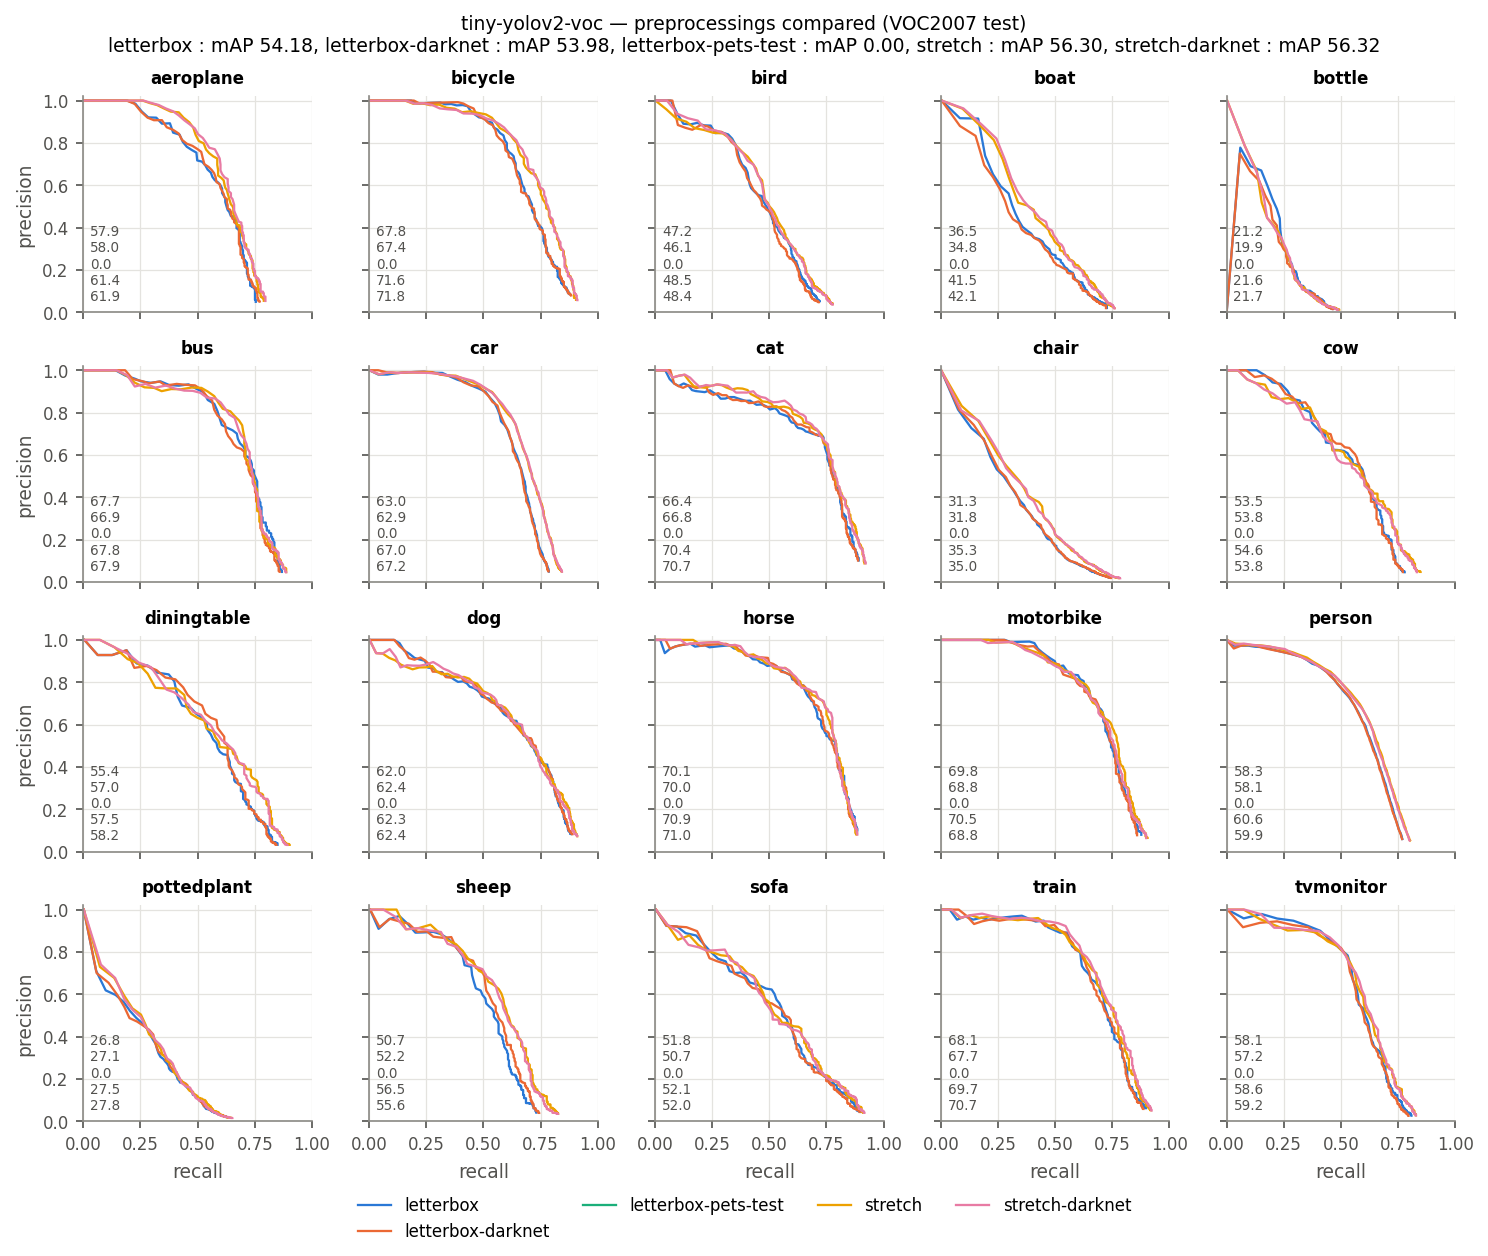
\includegraphics[width=\linewidth,height=0.42\textheight,keepaspectratio]{../../results/figures/resultats/pr_variantes.png}
\caption{Courbes précision-rappel par classe (11 points VOC07) pour chaque prétraitement évalué, puis les quatre superposées. (\texttt{pr})}
\label{fig:pr/pr_variantes}
% python -m tools.figures pr
\end{figure}}
\expandafter\def\csname artfig:nms_map\endcsname{%
\begin{figure}[htbp]
\centering
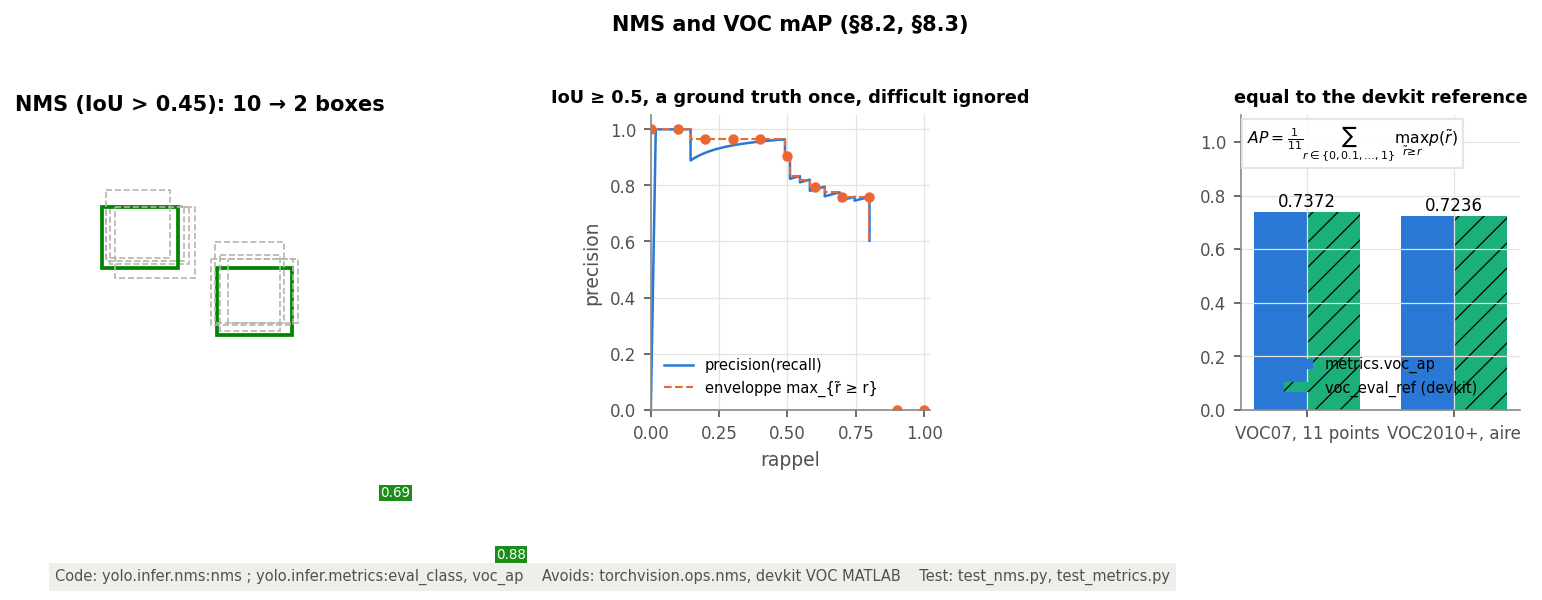
\includegraphics[width=\linewidth,height=0.42\textheight,keepaspectratio]{../../results/figures/maths/nms_map.png}
\caption{NMS pas à pas, appariement détections / vérités et courbe précision-rappel, AP VOC07 sur 11 points face à l'aire sous l'enveloppe, égale à la référence du devkit. (\texttt{nms\_map})}
\label{fig:nms_map}
% python -m tools.figures nms_map
\end{figure}}
\expandafter\def\csname artfig:quantification\endcsname{%
\begin{figure}[htbp]
\centering
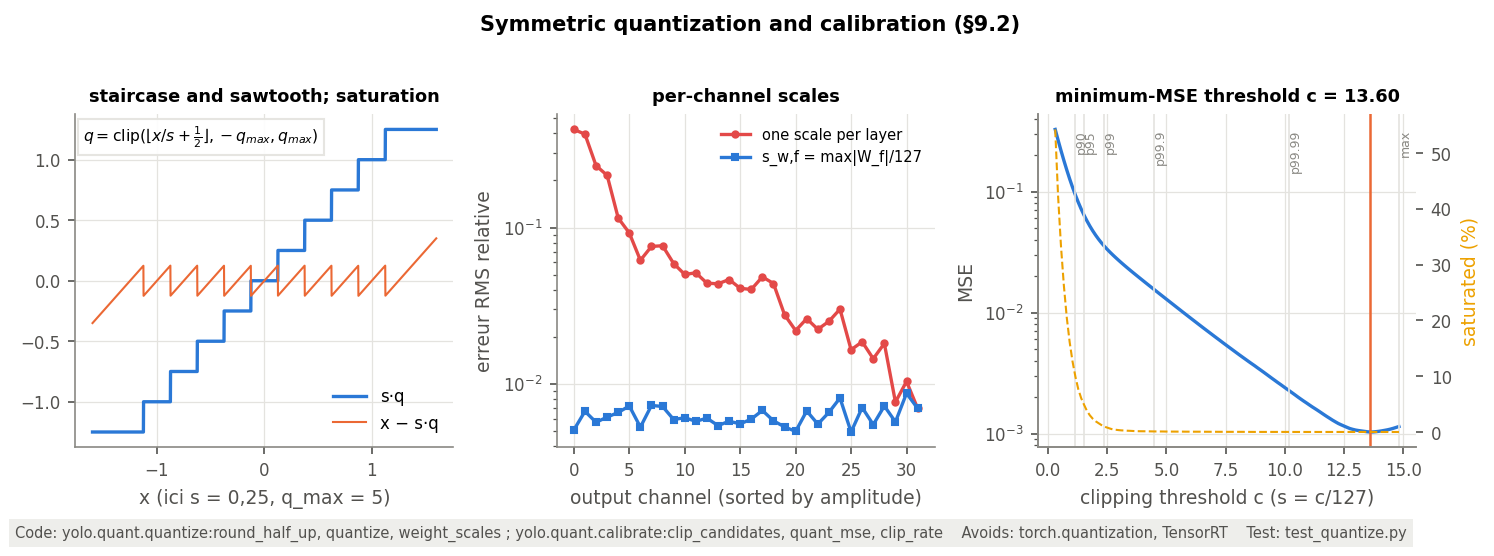
\includegraphics[width=\linewidth,height=0.42\textheight,keepaspectratio]{../../results/figures/maths/quantification.png}
\caption{Quantification symétrique : l'escalier et son erreur, échelles par canal face à une échelle par couche, choix du seuil d'écrêtage par la MSE. (\texttt{quantification})}
\label{fig:quantification}
% python -m tools.figures quantification
\end{figure}}
\expandafter\def\csname artfig:entier\endcsname{%
\begin{figure}[htbp]
\centering
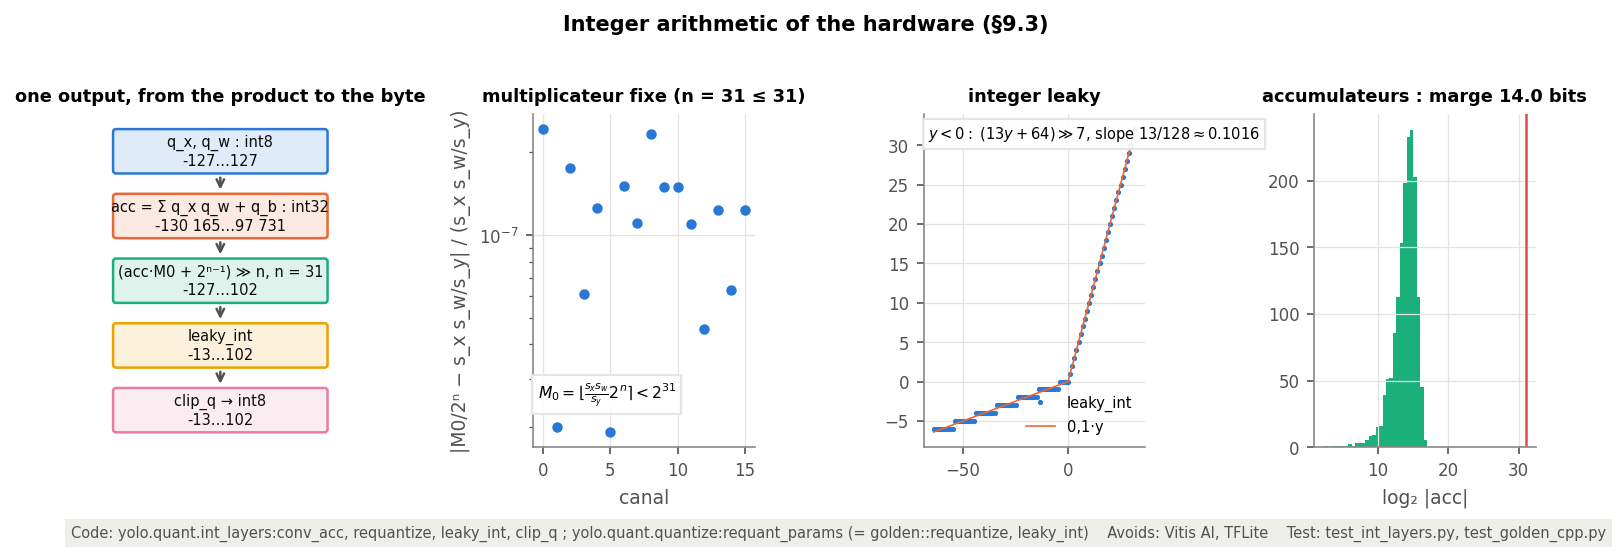
\includegraphics[width=\linewidth,height=0.42\textheight,keepaspectratio]{../../results/figures/maths/entier.png}
\caption{Arithmétique entière du matériel : chaîne d'une sortie, multiplicateur fixe M0/2$^n$, leaky entière 13/128 et marge des accumulateurs int32. (\texttt{entier})}
\label{fig:entier}
% python -m tools.figures entier
\end{figure}}
\expandafter\def\csname artfig:calibration/calibration_tiny-yolov2-voc\endcsname{%
\begin{figure}[htbp]
\centering
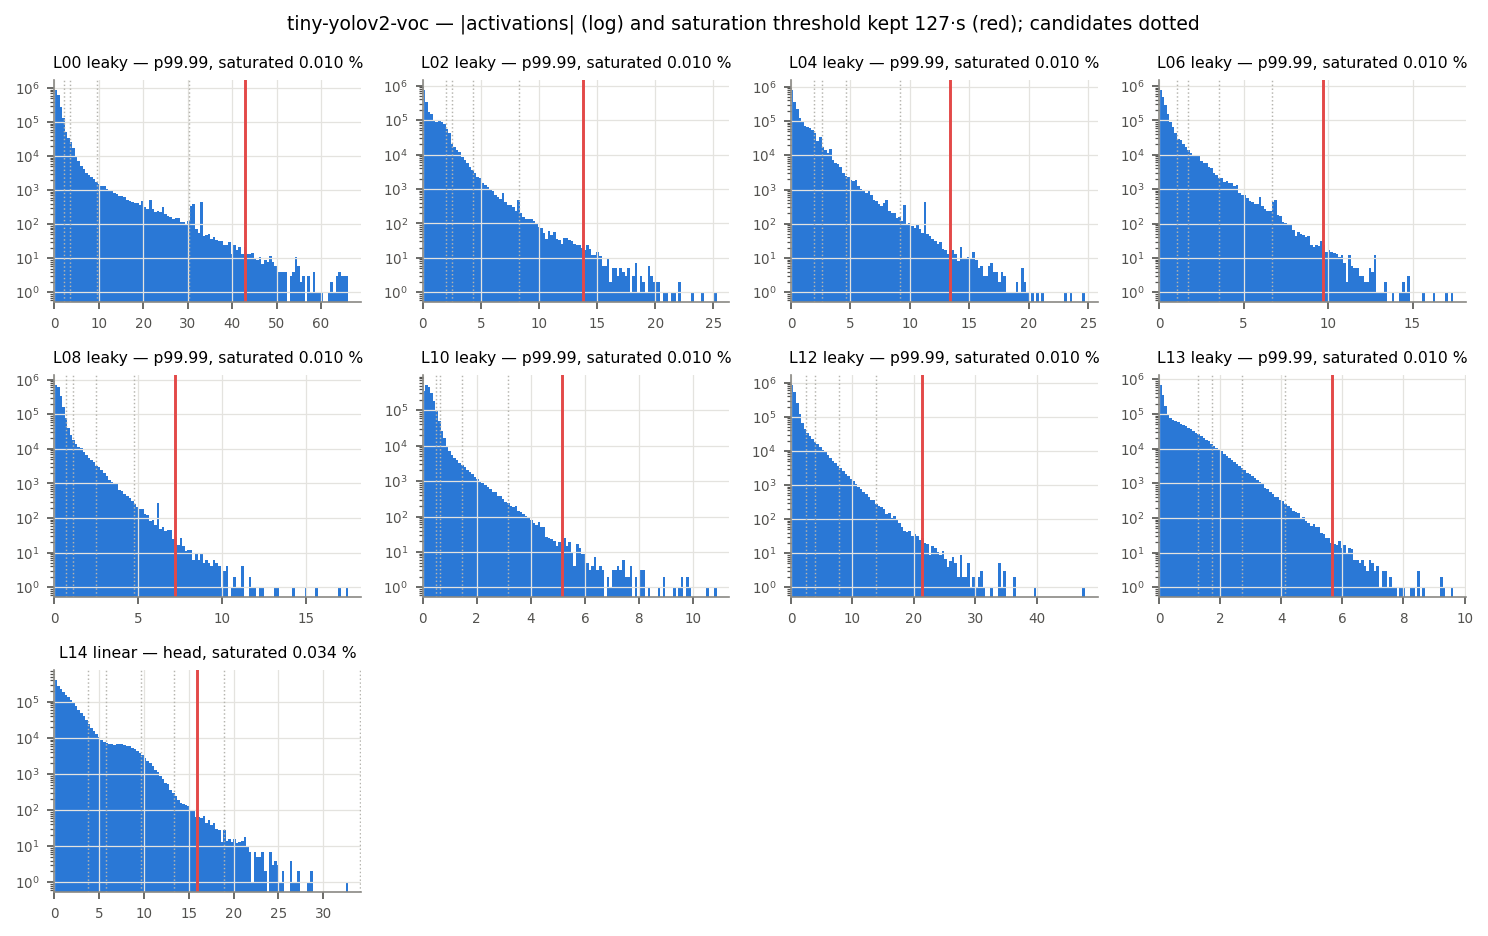
\includegraphics[width=\linewidth,height=0.42\textheight,keepaspectratio]{../../results/figures/resultats/calibration_tiny-yolov2-voc.png}
\caption{Distribution des activations par couche et seuil de saturation retenu par la calibration ; échelles des poids par canal. (\texttt{calibration})}
\label{fig:calibration/calibration_tiny-yolov2-voc}
% python -m tools.figures calibration
\end{figure}}
\expandafter\def\csname artfig:erreur_couches/erreur_couches_tiny-yolov2-voc\endcsname{%
\begin{figure}[htbp]
\centering
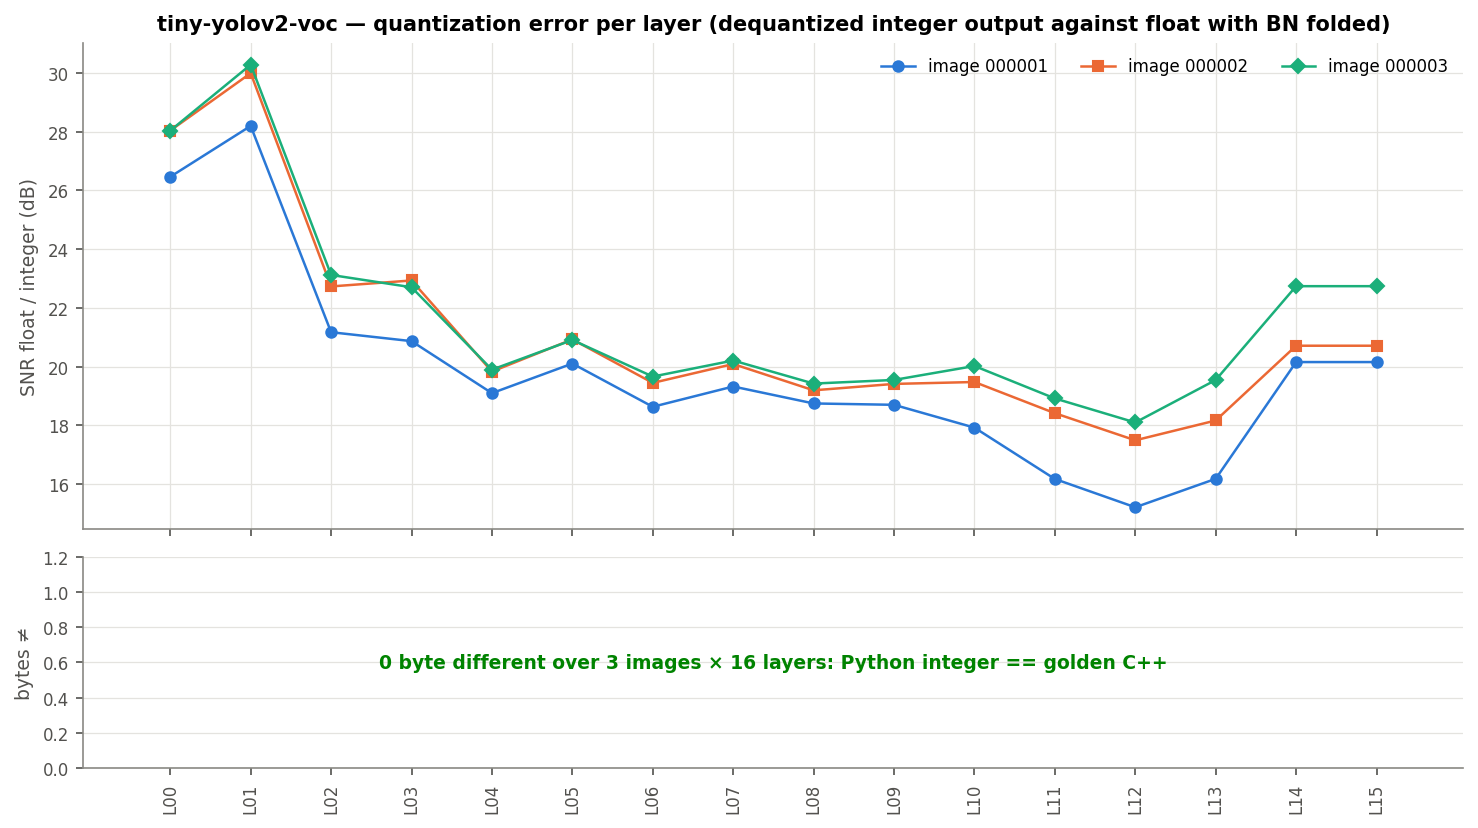
\includegraphics[width=\linewidth,height=0.42\textheight,keepaspectratio]{../../results/figures/resultats/erreur_couches_tiny-yolov2-voc.png}
\caption{SNR par couche entre le flottant et l'entier déquantifié, et écart entier Python $\leftrightarrow$ golden C++ (0 partout : bit-exact). (\texttt{erreur\_couches})}
\label{fig:erreur_couches/erreur_couches_tiny-yolov2-voc}
% python -m tools.figures erreur_couches
\end{figure}}
\expandafter\def\csname artfig:chaine_verif\endcsname{%
\begin{figure}[htbp]
\centering
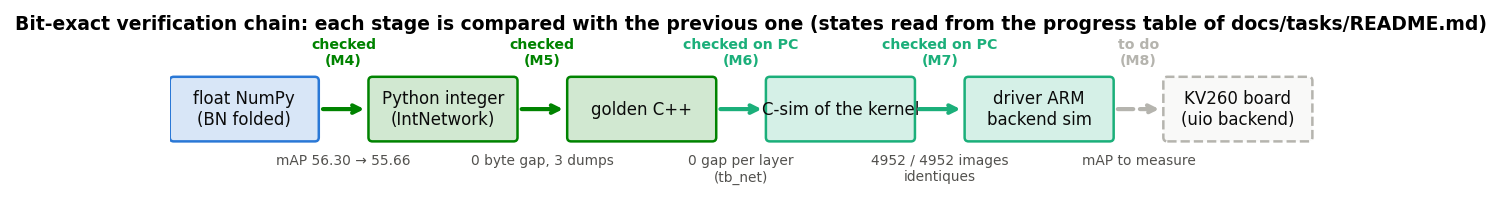
\includegraphics[width=\linewidth,height=0.42\textheight,keepaspectratio]{../../results/figures/materiel/chaine_verif.png}
\caption{Chaîne de vérification bit-exact, du flottant NumPy à la carte : critère et état de chaque passage. (\texttt{chaine\_verif})}
\label{fig:chaine_verif}
% python -m tools.figures chaine_verif
\end{figure}}
\expandafter\def\csname artfig:moteur\endcsname{%
\begin{figure}[htbp]
\centering
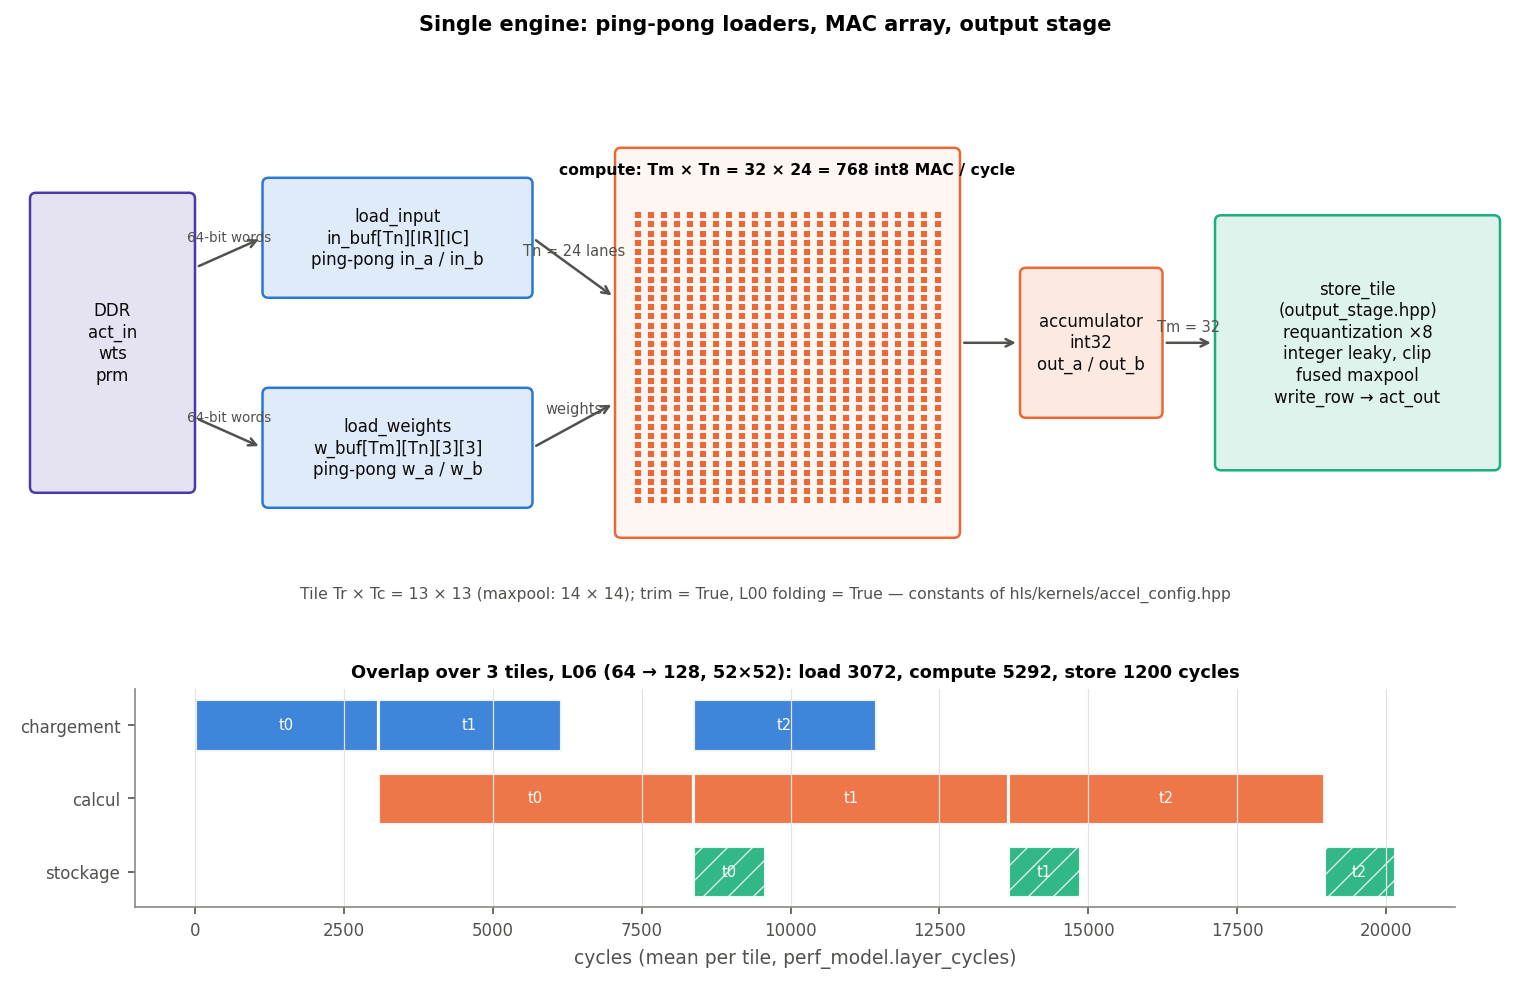
\includegraphics[width=\linewidth,height=0.42\textheight,keepaspectratio]{../../results/figures/materiel/moteur.png}
\caption{Moteur unique : chargeurs ping-pong, réseau Tm × Tn de MACs, accumulateur, étage de sortie, et chronogramme du recouvrement sur 3 tuiles. (\texttt{moteur})}
\label{fig:moteur}
% python -m tools.figures moteur
\end{figure}}
\expandafter\def\csname artfig:tuilage\endcsname{%
\begin{figure}[htbp]
\centering
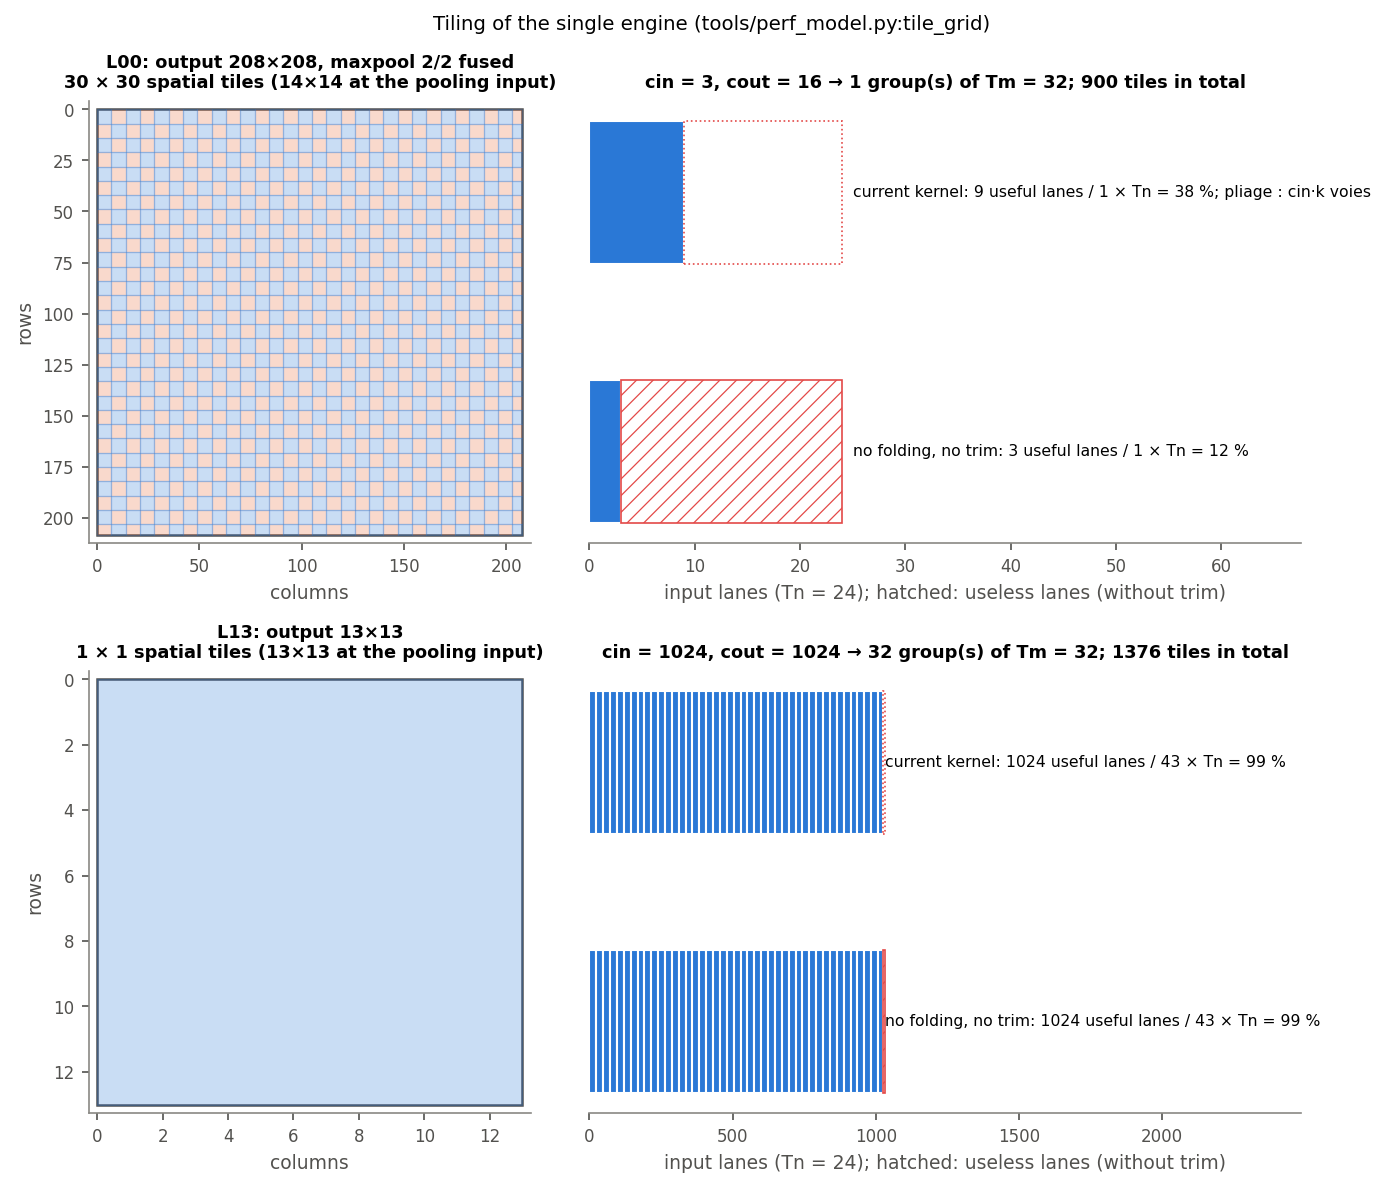
\includegraphics[width=\linewidth,height=0.42\textheight,keepaspectratio]{../../results/figures/materiel/tuilage.png}
\caption{Tuilage de deux couches : tuiles spatiales et voies d'entrée, avec le pliage de L00 (cin = 3) et la couche 13×13 couverte par une seule tuile. (\texttt{tuilage})}
\label{fig:tuilage}
% python -m tools.figures tuilage
\end{figure}}
\expandafter\def\csname artfig:soc\endcsname{%
\begin{figure}[htbp]
\centering
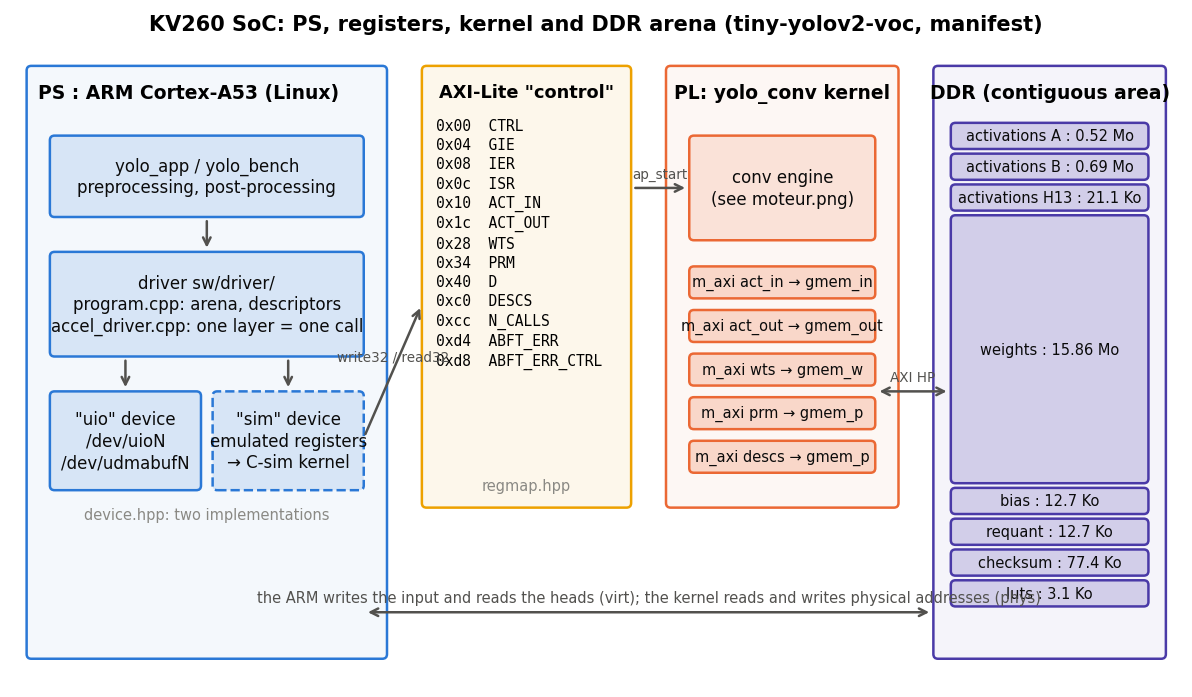
\includegraphics[width=\linewidth,height=0.42\textheight,keepaspectratio]{../../results/figures/materiel/soc.png}
\caption{Schéma du SoC : application et driver sur l'ARM, registres AXI-Lite, ports m\_axi du noyau et découpage de l'arène DDR. (\texttt{soc})}
\label{fig:soc}
% python -m tools.figures soc
\end{figure}}
\expandafter\def\csname artfig:cascade_m10\endcsname{%
\begin{figure}[htbp]
\centering
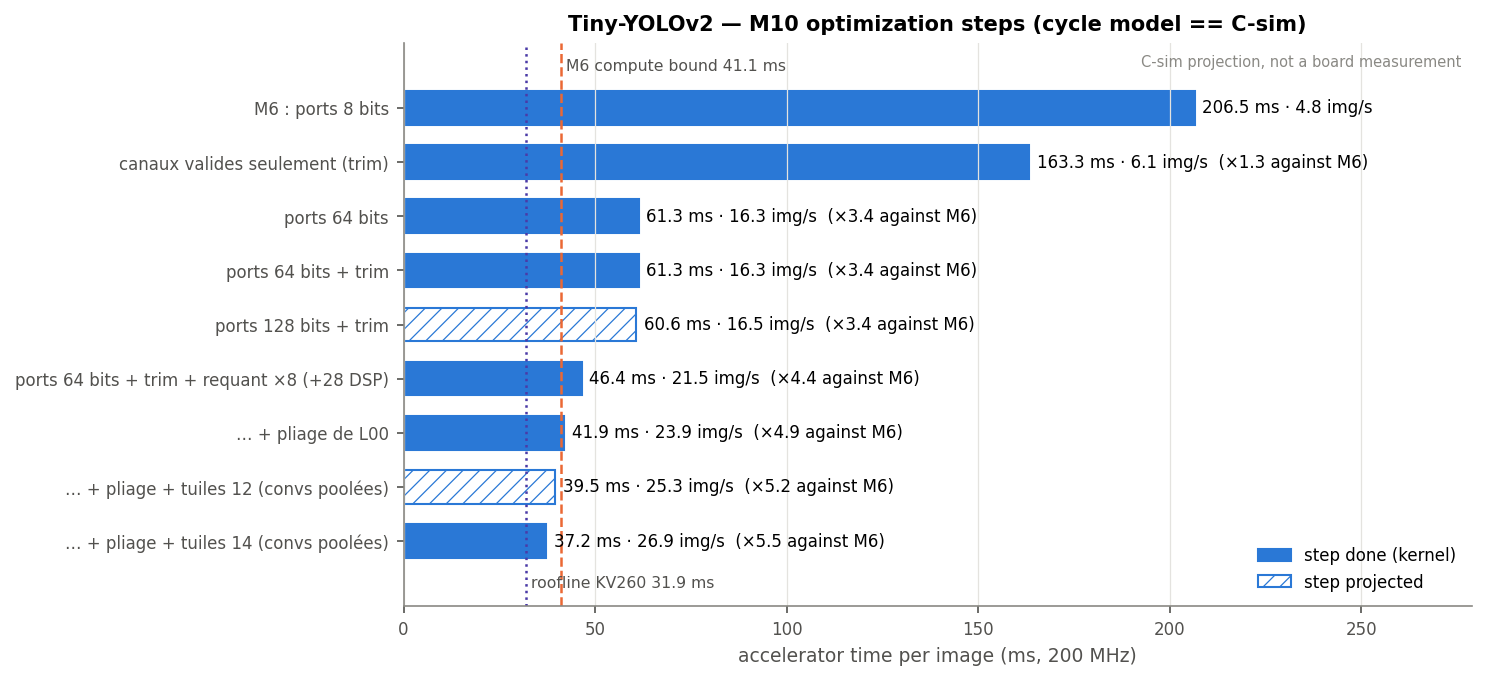
\includegraphics[width=\linewidth,height=0.42\textheight,keepaspectratio]{../../results/figures/resultats/cascade_m10.png}
\caption{Temps par image de Tiny-YOLOv2 à chaque piste d'optimisation M10, face à la borne de calcul et au roofline KV260. (\texttt{cascade\_m10})}
\label{fig:cascade_m10}
% python -m tools.figures cascade_m10
\end{figure}}
\expandafter\def\csname artfig:roofline_couches/roofline_couches_kv260\endcsname{%
\begin{figure}[htbp]
\centering
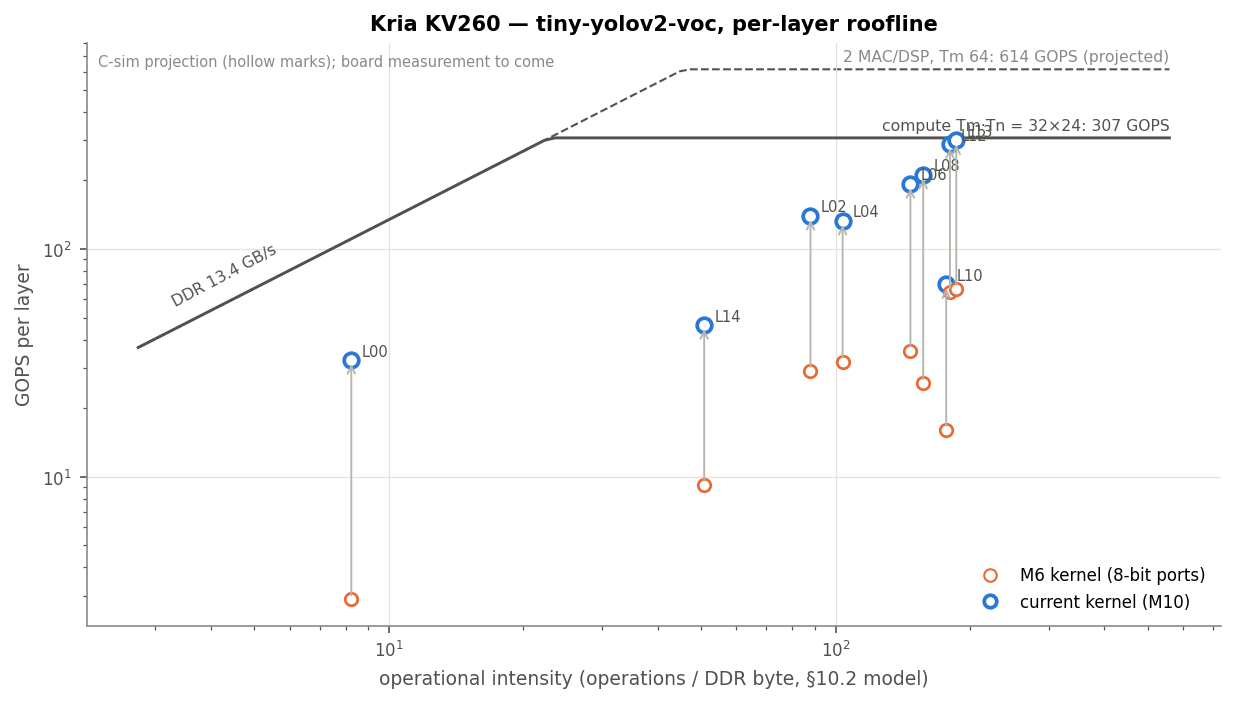
\includegraphics[width=\linewidth,height=0.42\textheight,keepaspectratio]{../../results/figures/resultats/roofline_couches_kv260.png}
\caption{Roofline KV260 avec un point par couche de Tiny-YOLOv2, avant et après les optimisations M10. (\texttt{roofline\_couches})}
\label{fig:roofline_couches/roofline_couches_kv260}
% python -m tools.figures roofline_couches
\end{figure}}
\expandafter\def\csname artfig:cycles_couches\endcsname{%
\begin{figure}[htbp]
\centering
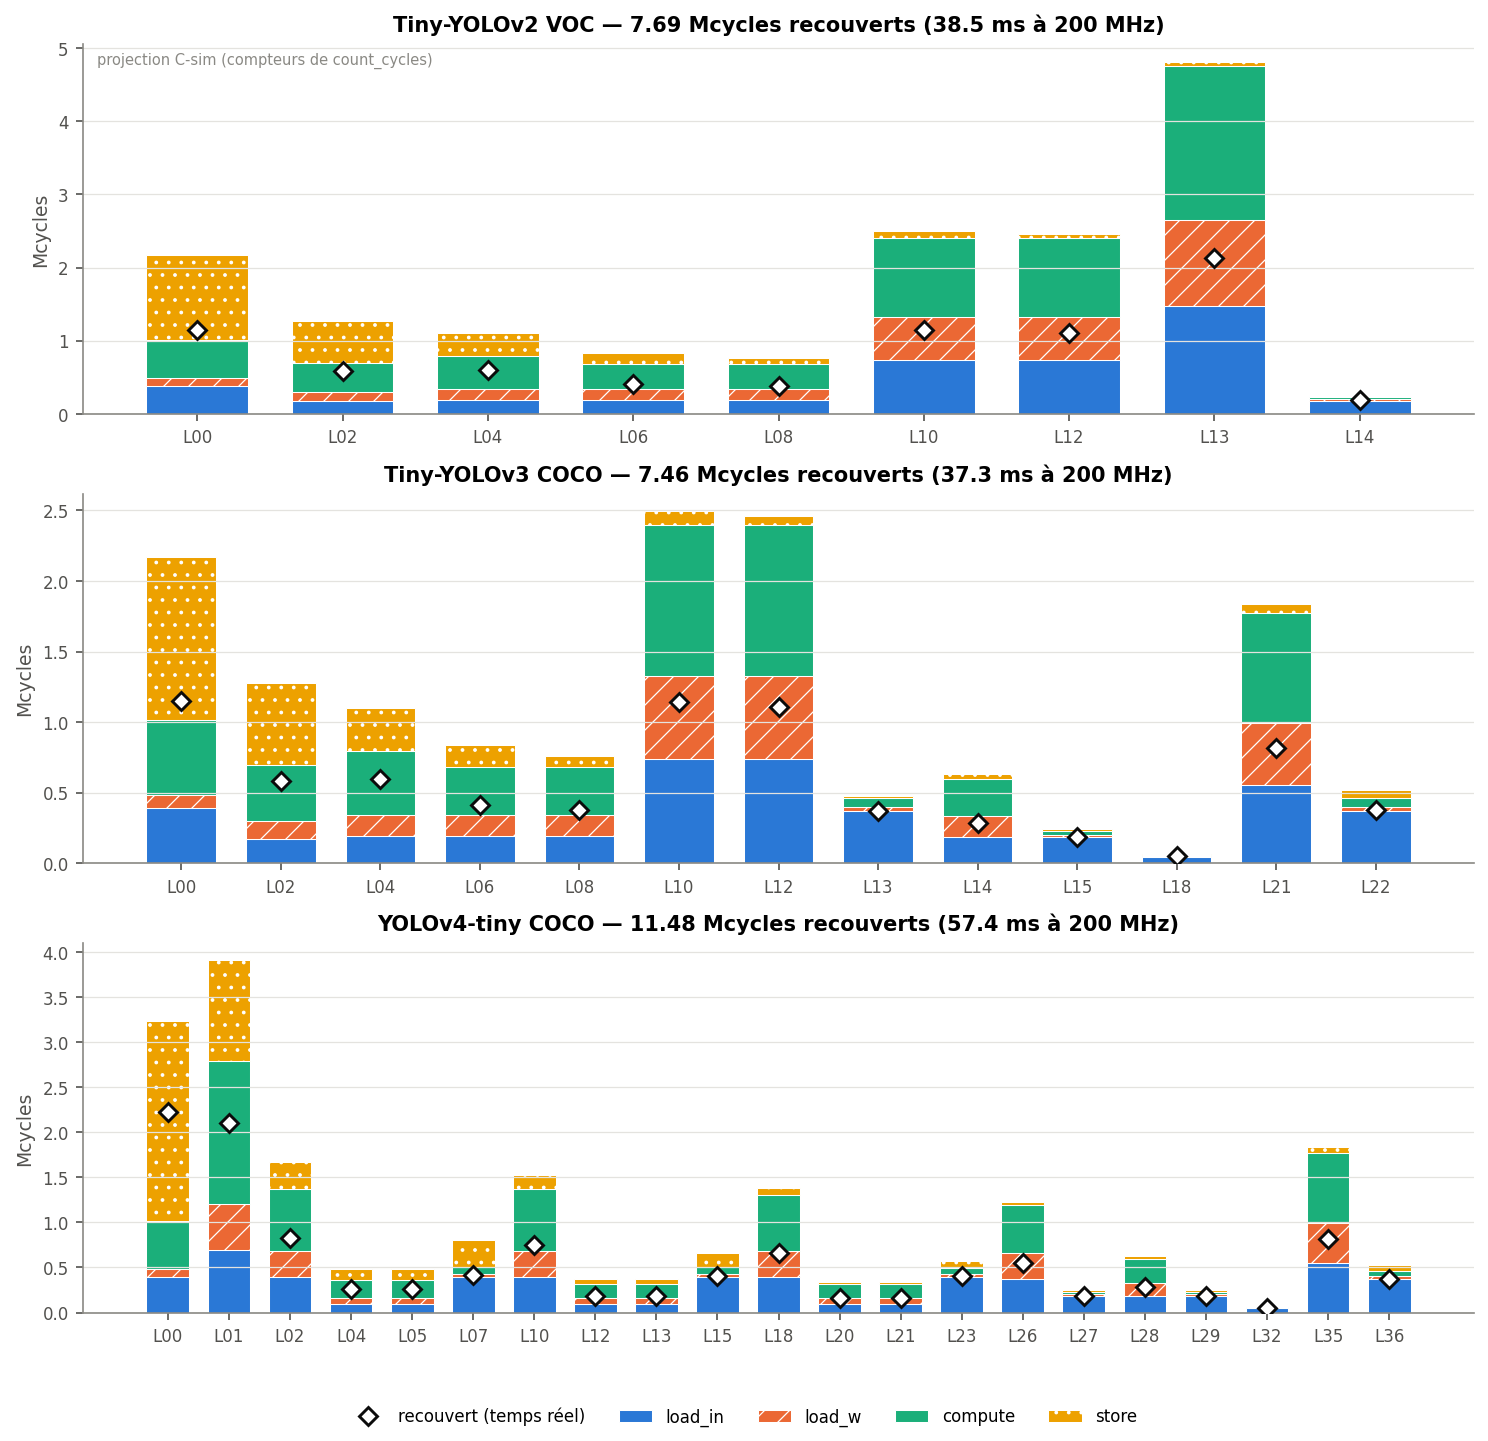
\includegraphics[width=\linewidth,height=0.42\textheight,keepaspectratio]{../../results/figures/resultats/cycles_couches.png}
\caption{Cycles par couche du noyau actuel, décomposés en chargements, calcul et stockage ; le losange donne le temps réel avec recouvrement. (\texttt{cycles\_couches})}
\label{fig:cycles_couches}
% python -m tools.figures cycles_couches
\end{figure}}
\expandafter\def\csname artfig:map_stades\endcsname{%
\begin{figure}[htbp]
\centering
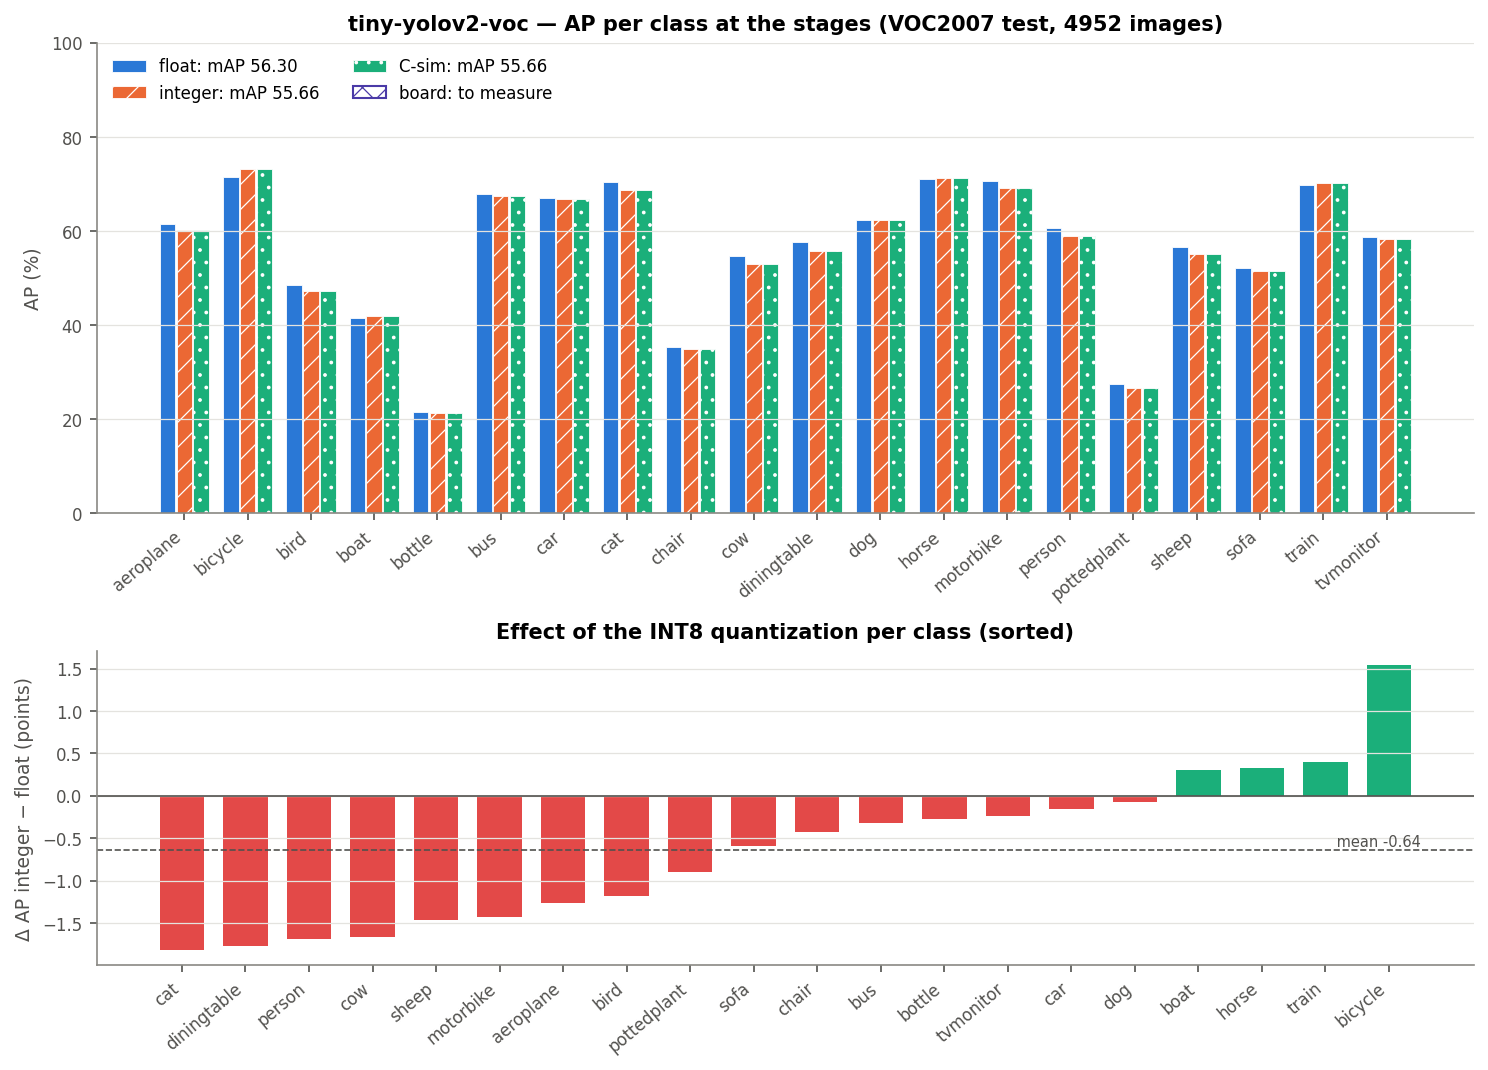
\includegraphics[width=\linewidth,height=0.42\textheight,keepaspectratio]{../../results/figures/resultats/map_stades.png}
\caption{AP par classe aux stades flottant, entier et C-sim (la carte quand elle sera mesurée), et écart entier − flottant trié. (\texttt{map\_stades})}
\label{fig:map_stades}
% python -m tools.figures map_stades
\end{figure}}
\expandafter\def\csname artfig:ressources\endcsname{%
\begin{figure}[htbp]
\centering
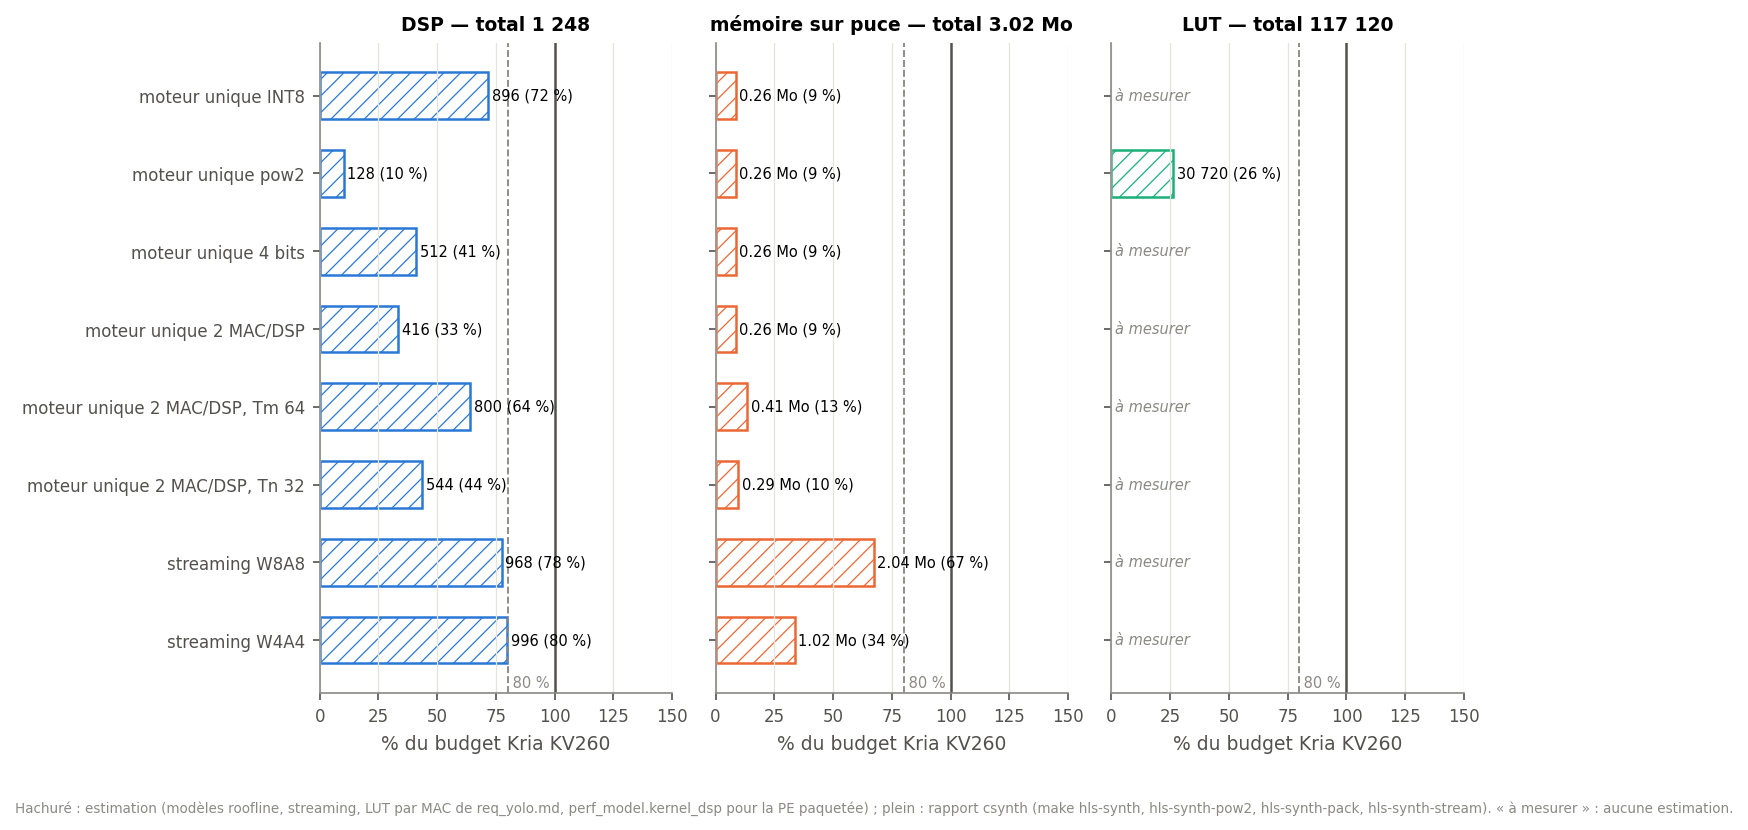
\includegraphics[width=\linewidth,height=0.42\textheight,keepaspectratio]{../../results/figures/resultats/ressources.png}
\caption{DSP, mémoire sur puce et LUT des architectures (moteur unique INT8, pow2 et 4 bits, streaming) face au budget de la KV260 ; hachuré : estimation, plein : synthèse. (\texttt{ressources})}
\label{fig:ressources}
% python -m tools.figures ressources
\end{figure}}
\expandafter\def\csname artfig:hw_postproc\endcsname{%
\begin{figure}[htbp]
\centering
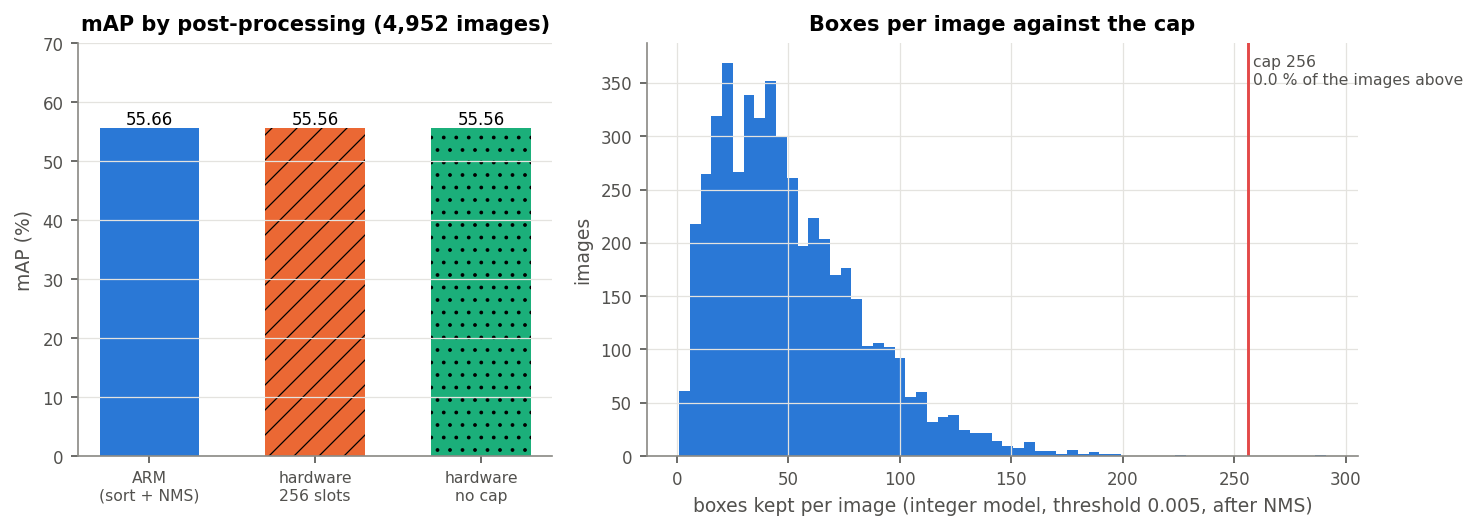
\includegraphics[width=\linewidth,height=0.42\textheight,keepaspectratio]{../../results/figures/resultats/hw_postproc.png}
\caption{mAP avec le post-traitement matériel, avec et sans plafond de boîtes, et nombre de boîtes par image face au plafond. (\texttt{hw\_postproc})}
\label{fig:hw_postproc}
% python -m tools.figures hw_postproc
\end{figure}}
\expandafter\def\csname artfig:map_formats\endcsname{%
\begin{figure}[htbp]
\centering
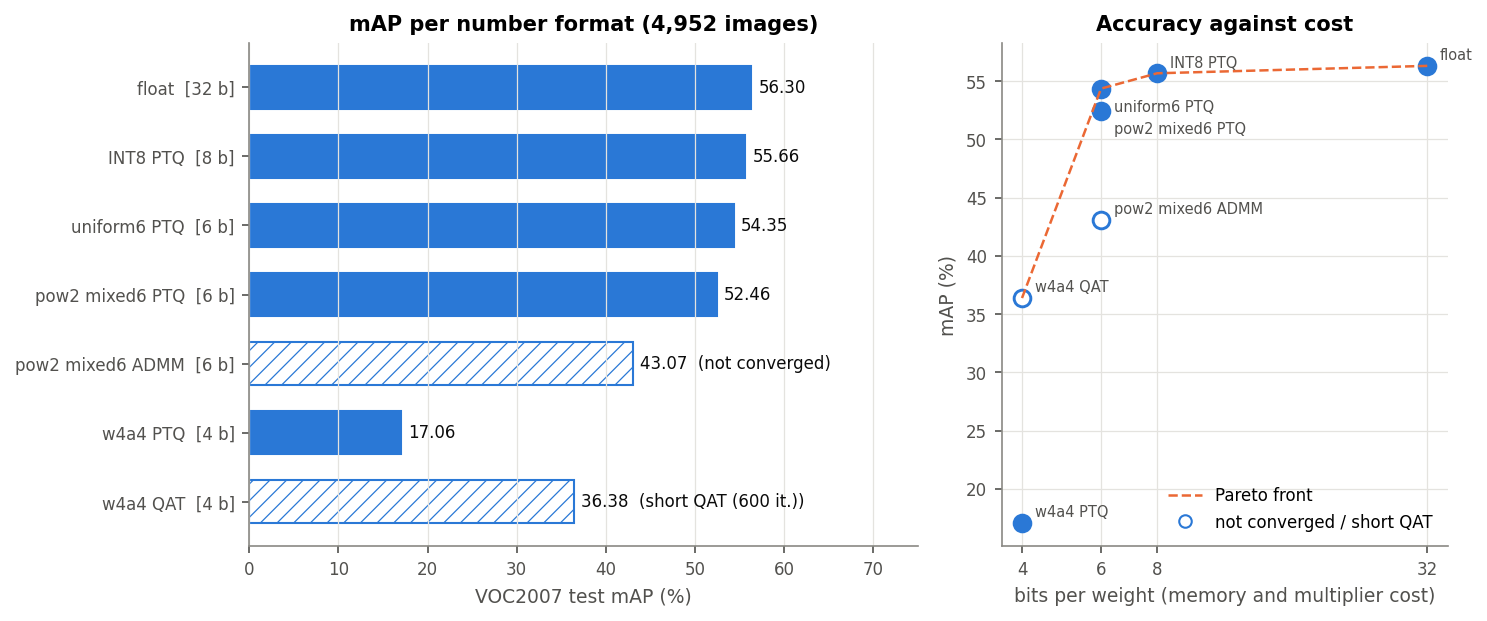
\includegraphics[width=\linewidth,height=0.42\textheight,keepaspectratio]{../../results/figures/resultats/map_formats.png}
\caption{mAP de Tiny-YOLOv2 selon le format des poids (flottant, INT8, puissances de 2, 4 bits), et frontière précision / bits. (\texttt{map\_formats})}
\label{fig:map_formats}
% python -m tools.figures map_formats
\end{figure}}
\expandafter\def\csname artfig:streaming\endcsname{%
\begin{figure}[htbp]
\centering
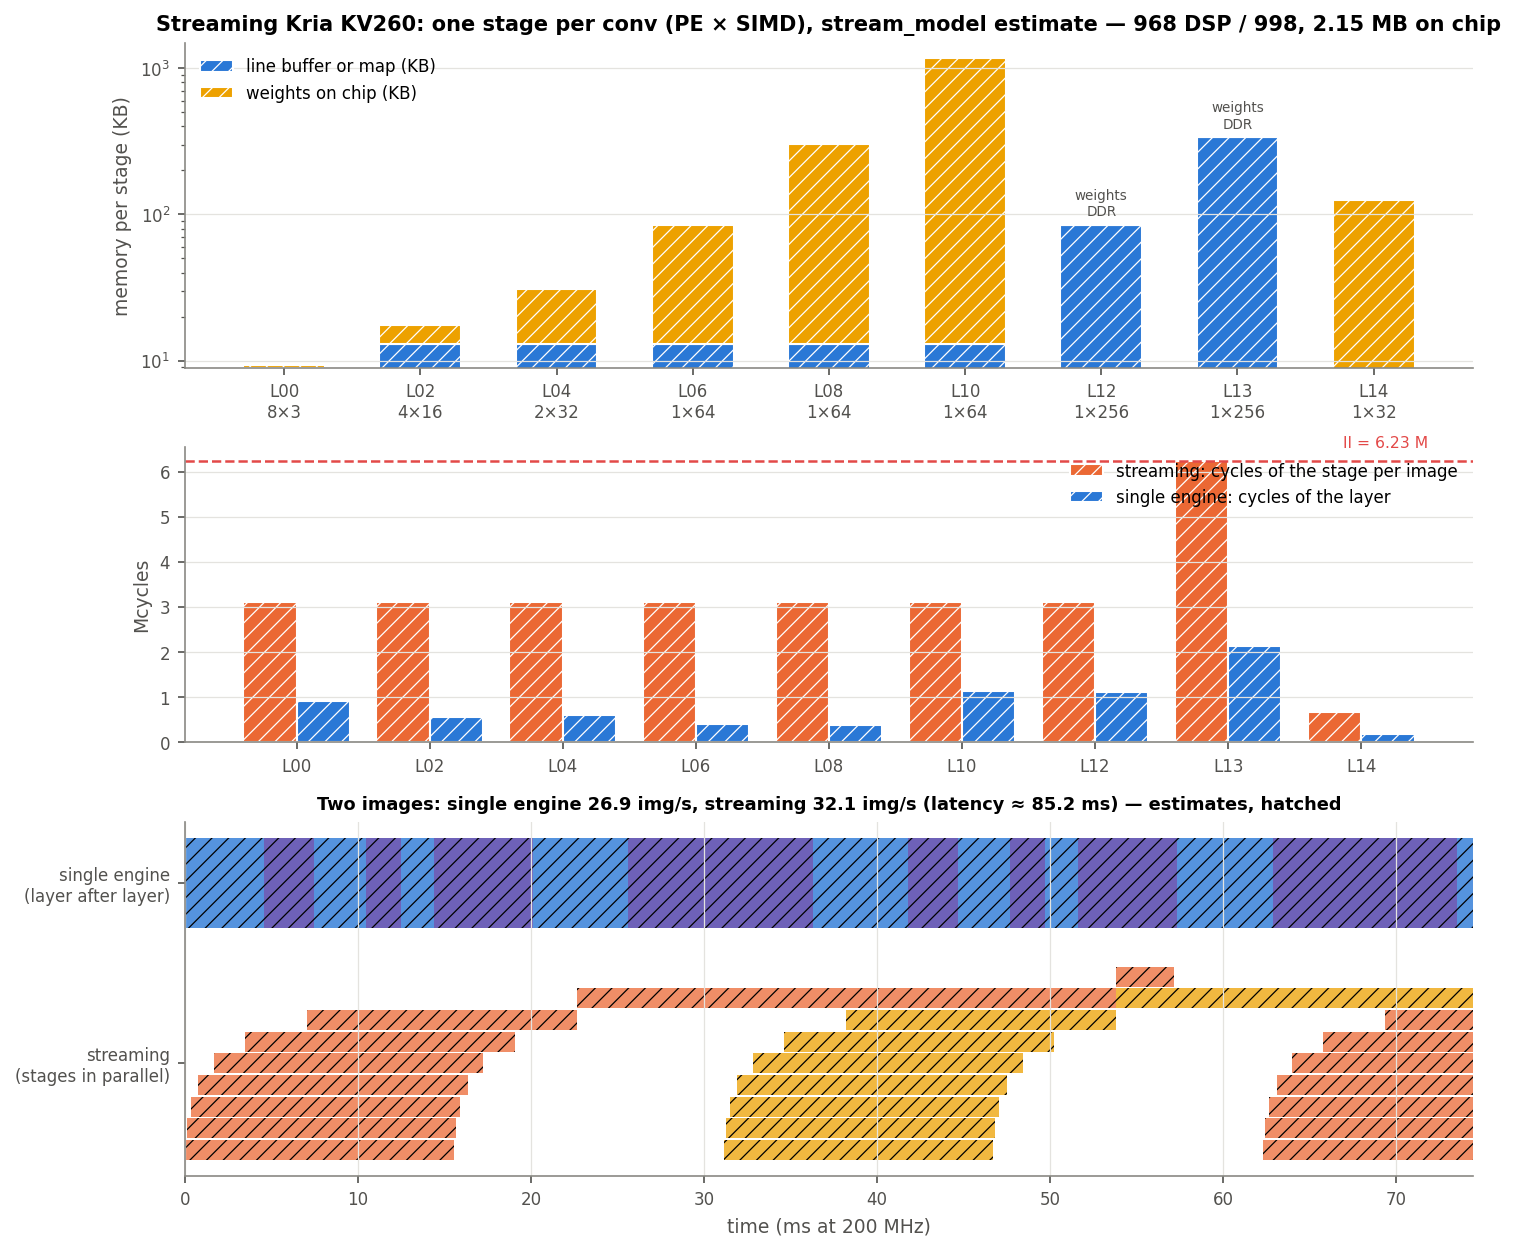
\includegraphics[width=\linewidth,height=0.42\textheight,keepaspectratio]{../../results/figures/materiel/streaming.png}
\caption{Architecture streaming face au moteur unique : mémoire et parallélisme par étage, cycles par couche, chronogramme sur deux images (estimations). (\texttt{streaming})}
\label{fig:streaming}
% python -m tools.figures streaming
\end{figure}}
\expandafter\def\csname artfig:detections\endcsname{%
\begin{figure}[htbp]
\centering
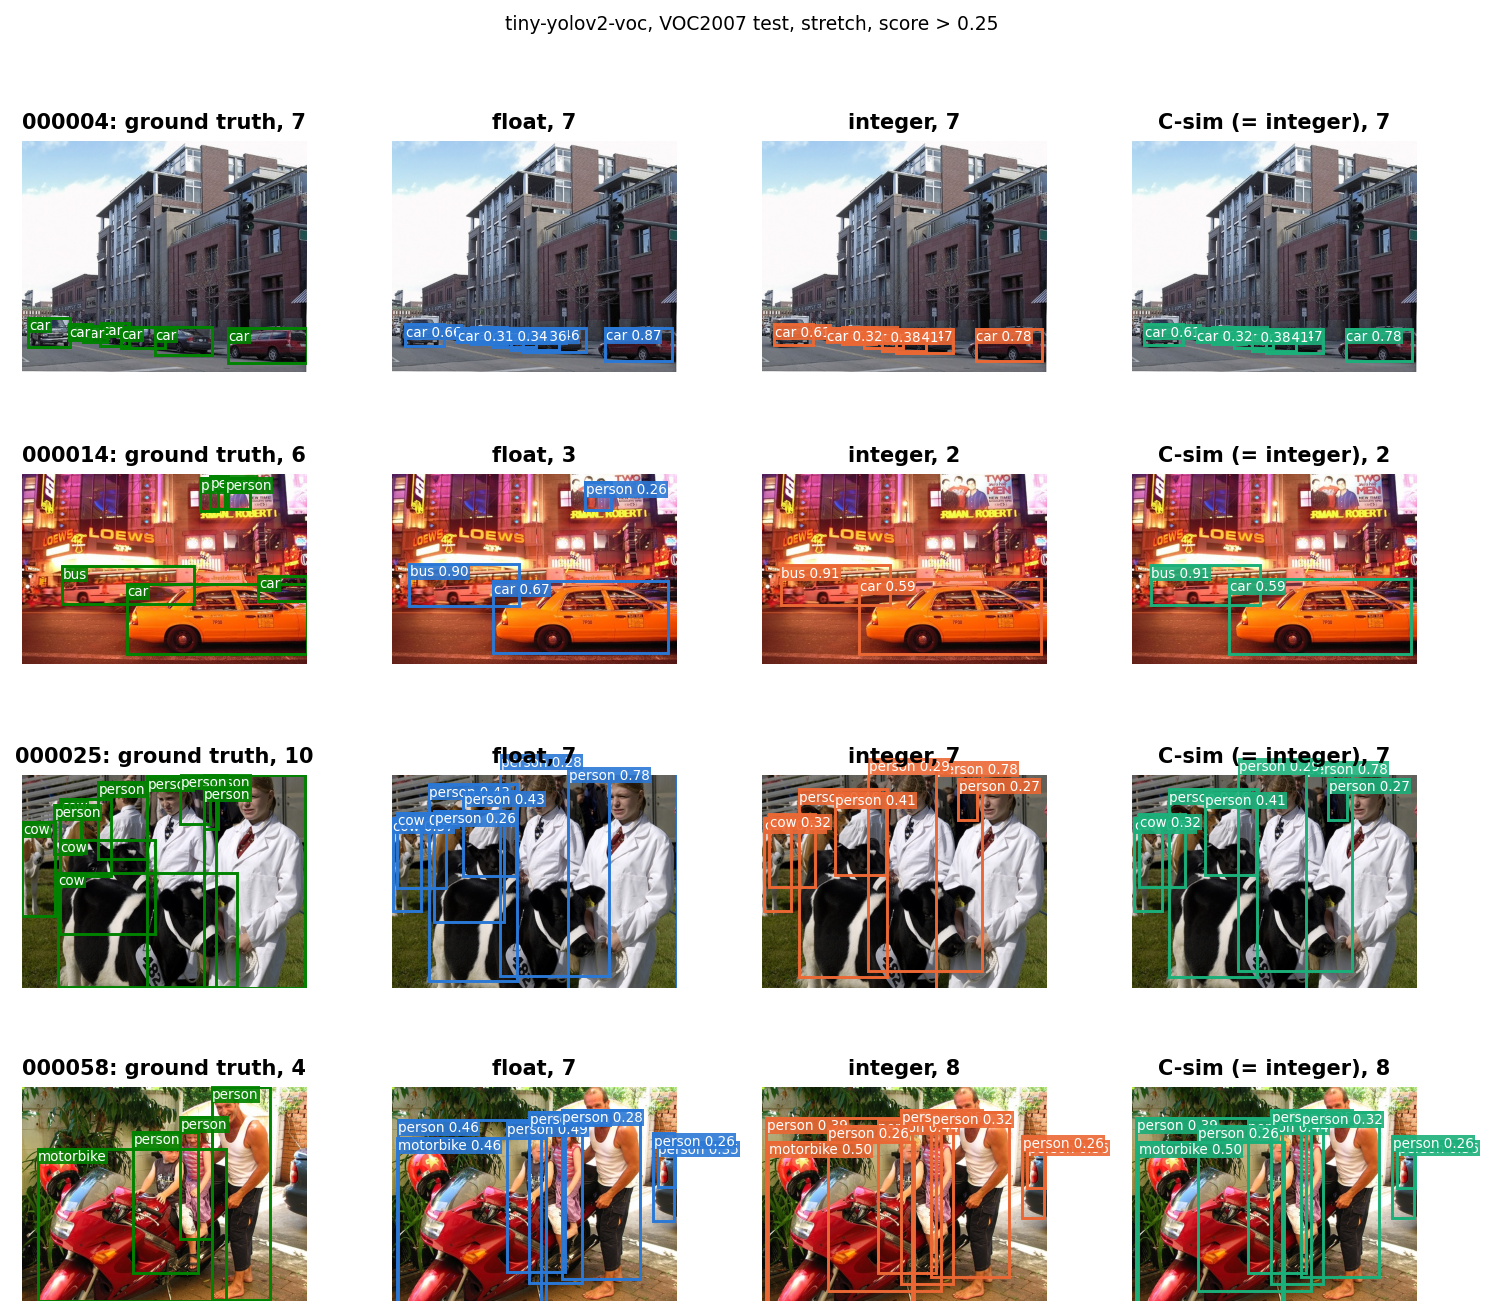
\includegraphics[width=\linewidth,height=0.42\textheight,keepaspectratio]{../../results/figures/resultats/detections.png}
\caption{Vérité terrain, flottant, entier et C-sim sur quatre images de VOC2007 test : les colonnes entier et C-sim sont identiques. (\texttt{detections})}
\label{fig:detections}
% python -m tools.figures detections
\end{figure}}
\expandafter\def\csname artfig:tests\endcsname{%
\begin{figure}[htbp]
\centering
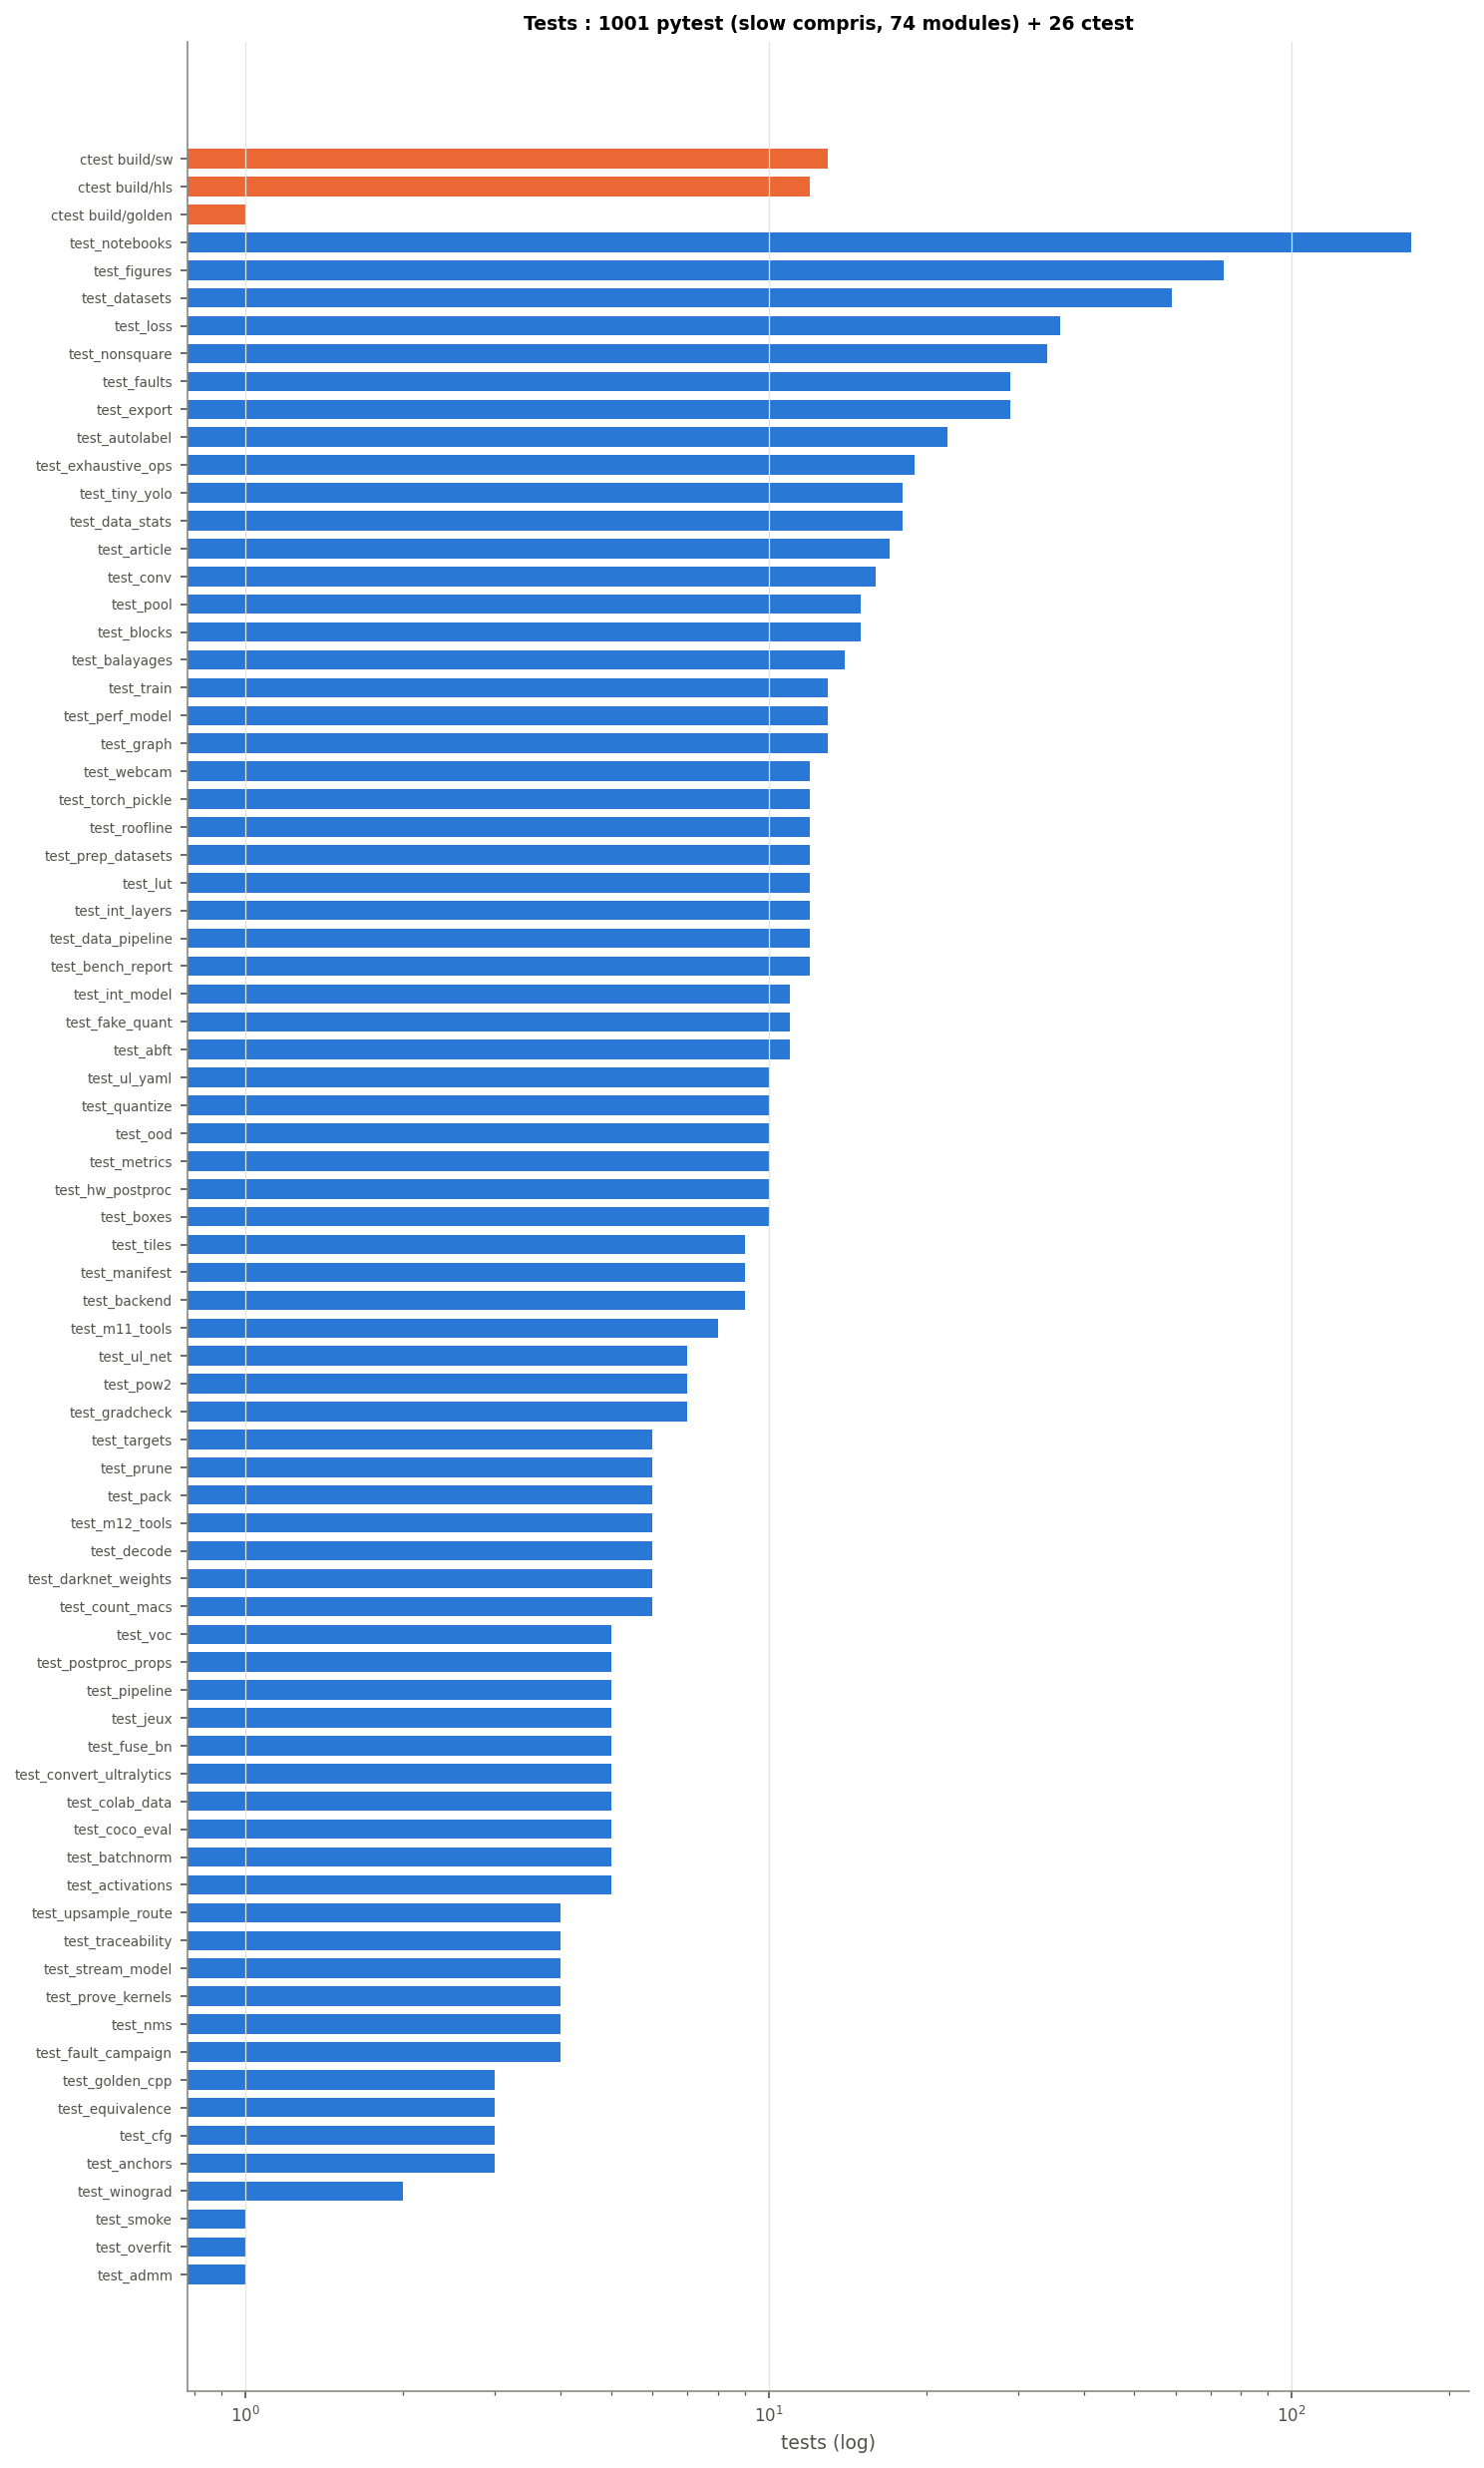
\includegraphics[width=\linewidth,height=0.42\textheight,keepaspectratio]{../../results/figures/projet/tests.png}
\caption{Nombre de tests par module Python (pytest, slow compris) et par build C++ (ctest), et leur durée quand \texttt{make test-durations} a été lancé. (\texttt{tests})}
\label{fig:tests}
% python -m tools.figures tests
\end{figure}}
\expandafter\def\csname artfig:code\endcsname{%
\begin{figure}[htbp]
\centering
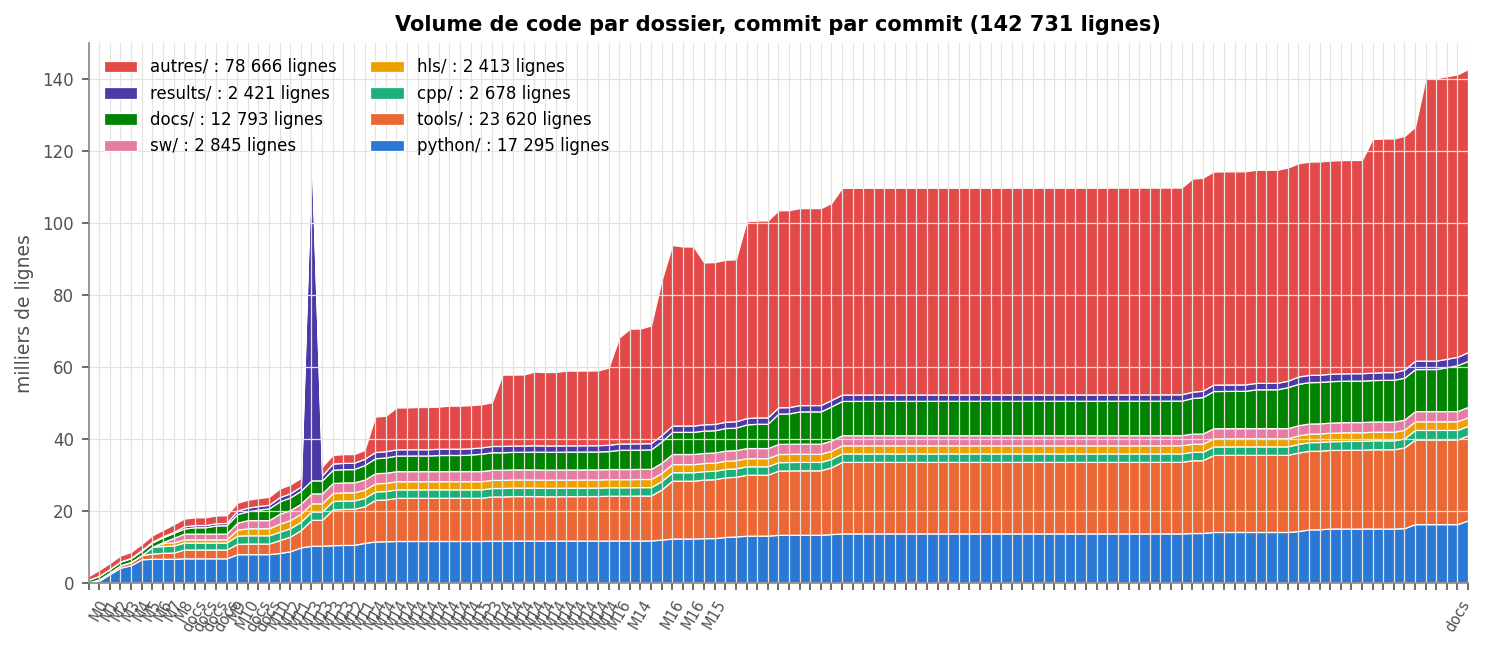
\includegraphics[width=\linewidth,height=0.42\textheight,keepaspectratio]{../../results/figures/projet/code.png}
\caption{Lignes par dossier (python, tools, cpp, hls, sw, docs, results) commit par commit. (\texttt{code})}
\label{fig:code}
% python -m tools.figures code
\end{figure}}
% ---- milestones, pending keys, revision
\newcommand\articleetat{%
\begin{tabular}{@{}lrrr@{}}
\toprule
\textbf{Milestone} & \textbf{Tasks} & \textbf{Done} & \textbf{Progress} \\
\midrule
M0 & 6 & 6 & 100\,\% \\
M1 & 9 & 8 & 89\,\% \\
M2 & 9 & 8 & 89\,\% \\
M3 & 4 & 4 & 100\,\% \\
M4 & 7 & 7 & 100\,\% \\
M5 & 6 & 6 & 100\,\% \\
M6 & 6 & 1 & 17\,\% \\
M7 & 4 & 0 & 0\,\% \\
M8 & 3 & 0 & 0\,\% \\
M9 & 1 & 0 & 0\,\% \\
M9.1 & 3 & 2 & 67\,\% \\
M9.2 & 4 & 3 & 75\,\% \\
M9.3 & 6 & 5 & 83\,\% \\
M9.4 & 3 & 3 & 100\,\% \\
M10 & 14 & 0 & 0\,\% \\
M12 & 11 & 0 & 0\,\% \\
M11 & 8 & 1 & 12\,\% \\
M13 & 54 & 54 & 100\,\% \\
M14 & 12 & 8 & 67\,\% \\
M15 & 16 & 1 & 6\,\% \\
M16 & 20 & 18 & 90\,\% \\
M17 & 21 & 17 & 81\,\% \\
M18 & 11 & 9 & 82\,\% \\
M19 & 12 & 5 & 42\,\% \\
M20 & 10 & 9 & 90\,\% \\
M21 & 12 & 6 & 50\,\% \\
M22 & 10 & 9 & 90\,\% \\
M23 & 6 & 0 & 0\,\% \\
M24 & 6 & 0 & 0\,\% \\
M25 & 6 & 0 & 0\,\% \\
M26 & 6 & 0 & 0\,\% \\
\midrule
\textbf{Total} & \textbf{306} & \textbf{190} & \textbf{62\,\%} \\
\bottomrule
\end{tabular}}
\newcommand\articleetatresume{190 of 306 tasks done across 31 milestones, 6 milestones complete}
\newcommand\articlestatuslist{%
{\raggedright
\begin{itemize}
\item \textbf{projection} (10): \texttt{perf.cascade}, \texttt{perf.kv260}, \texttt{perf.kv260.bound.ms}, \texttt{perf.kv260.m6.ms}, \texttt{perf.kv260.roofline.ms}, \texttt{perf.kv260.v2.eff}, \texttt{perf.kv260.v2.fps}, \texttt{perf.kv260.v2.gops}, \texttt{perf.kv260.v2.ms}, \texttt{perf.kv260.v3.ms}
\item \textbf{estimate} (4): \texttt{stream.w4.fps}, \texttt{stream.w8.dsp}, \texttt{stream.w8.fps}, \texttt{stream.w8.latency}
\item \textbf{tier-R} (9): \texttt{balayage.crowdhuman.meilleur.map}, \texttt{balayage.exdark.meilleur.map}, \texttt{balayage.flir.meilleur.map}, \texttt{balayage.kitti.meilleur.map}, \texttt{balayage.visdrone.meilleur.map}, \texttt{balayage.voc.meilleur.map}, \texttt{balayages.meilleurs}, \texttt{quant.sensitive.gap}, \texttt{quant.sensitive.layer}
\item \textbf{csim} (3): \texttt{map.voc.csim}, \texttt{map.voc.identical}, \texttt{verif.hwpp.cases}
\end{itemize}\par}}
\newcommand\articlerev{rev.~\texttt{66f9001-dirty}, 2026-10-19}


\graphicspath{{../../results/figures/}}
% \fig{path}{height as a fraction of the text height}
\newcommand\fig[2]{{\centering\includegraphics[width=\linewidth,height=#2\textheight,keepaspectratio]{#1}\par}}
\newcommand\src[1]{\par\vfill{\tiny\color{gray}source: \texttt{#1}}}
\newcommand\proj{\textcolor{orange!80!black}{\small(projection, not measured)}}
\newcommand\plan{\textcolor{orange!80!black}{\small(estimates)}}
\newcommand\done{\textcolor{mLightGreen!80!black}{\textbf{done}}}
\newcommand\todo{\textcolor{orange!80!black}{\textbf{open}}}
% \repolink{path in the GitHub repository}{text}
\newcommand\repolink[2]{\href{https://github.com/lrivals/EmbeddedComputervision/#1}{\textcolor{mLightBrown!80!black}{\texttt{#2}}}}

\title{Embedded YOLO from scratch}
\subtitle{Status, current results and the next training and test campaigns}
\author{Léonard Rivals}
\date{22 October 2026}

\begin{document}

\maketitle

\begin{frame}{In three points}
  \begin{columns}[T]
    \column{0.32\textwidth}
    \begin{block}{Where we are}
      \small
      The PC side of the chain is complete and bit-exact for four networks.
      Safety evidence (equivalence, ABFT, latency bound) is in place.
      The board is not available yet.
    \end{block}
    \column{0.32\textwidth}
    \begin{block}{What we measured}
      \small
      VOC: \chiffre{map.voc.float} float $\to$ \chiffre{map.voc.int8} INT8 $\to$
      \chiffre{map.voc.csim}.
      COCO v4-tiny: \chiffre{map.coco.v4.ap50} $\to$ \chiffre{map.coco.v4.int8.ap50} AP50.
      KV260: \chiffre{perf.kv260.v2.ms}\,ms per image.
    \end{block}
    \column{0.32\textwidth}
    \begin{block}{What is left to run}
      \small
      $\approx$\,40\,h of PC CPU, $\approx$\,12\,h of C-sim and $\approx$\,110--120\,h of Colab
      GPU. Four transfers unblock most of it.
    \end{block}
  \end{columns}
\end{frame}

% =====================================================================================
\section{Where we are}

\begin{frame}{Progress by milestone}
  \begin{columns}[T]
    \column{0.40\textwidth}
    \centering\tiny\renewcommand\arraystretch{0.68}%
    \scalebox{0.72}{\articleetat}
    \column{0.58\textwidth}
    \fig{projet/avancement.png}{0.75}
  \end{columns}
\end{frame}

\begin{frame}{The chain today}
  \centering
  \begin{tikzpicture}[node distance=4mm and 4mm, every node/.style={font=\scriptsize},
      ok/.style={draw, rounded corners, fill=mLightGreen!25, minimum height=9mm, align=center, text width=1.75cm},
      hw/.style={ok, fill=black!8, dashed},
      arr/.style={-{Stealth}, thick}]
    \node[ok] (np) {NumPy float\\fwd + bwd};
    \node[ok, right=of np] (int) {INT8 integer\\model};
    \node[ok, right=of int] (gold) {golden C++};
    \node[ok, right=of gold] (cs) {HLS C-sim\\+ ARM driver};
    \node[hw, right=of cs] (co) {synthesis,\\co-sim};
    \node[hw, right=of co] (bd) {KV260\\board};
    \foreach \a/\b in {np/int, int/gold, gold/cs, cs/co, co/bd} \draw[arr] (\a) -- (\b);
  \end{tikzpicture}

  \medskip
  \scriptsize
  \begin{tabularx}{\linewidth}{@{}l>{\raggedright\arraybackslash}Xl@{}}
    \toprule
    Network & PC chain & Next \\
    \midrule
    Tiny-YOLOv2 VOC & float, int, golden, C-sim: identical on 4,952 images & board \\
    Tiny-YOLOv3 COCO & identical up to C-sim (20 images) & full COCO C-sim pass \\
    YOLOv4-tiny COCO & identical up to C-sim (20 images, smoke run 10) & full C-sim, QAT \\
    YOLOv7-tiny COCO & exported, calibrated; 34.3 AP at 416 (paper 35.2) & C-sim pass, VOC training \\
    YOLOv5n COCO & torch-free, 28.1 AP at 640 (published 28.0); trainable & VOC training, integer \\
    YOLOv8n COCO & torch-free reader & mAP, training (M35) \\
    \bottomrule
  \end{tabularx}

  \medskip
  \colorbox{mLightGreen!25}{done on the PC}\quad
  \colorbox{black!8}{needs Vitis / board, parked in \texttt{docs/tasks/deferred/}}
  \src{results/equivalence.md, results/map\_stades.md, docs/tasks/M33-yolov5n.md}
\end{frame}

\begin{frame}{Since the last deck (20 October)}
  \footnotesize
  \begin{columns}[T]
    \column{0.5\textwidth}
    \textbf{Finished}
    \begin{itemize}
      \item \textbf{M28 equivalence}: matrix per layer and stage, exhaustive operator tests,
        z3 proof of the scalar kernels, traceability checked in CI, tool-chain risks,
        post-processing properties (6 / 7, board row left)
      \item \textbf{M30}: static latency bound of the accelerator (T30.0)
      \item \textbf{M32}: Oxford-IIIT Pet boxed from the trimaps, datasheets
      \item \textbf{M33}: \texttt{.pt} read without torch, network from the Ultralytics
        YAML, C3 / SPPF in forward and backward; v5 decoding (28.1 AP), targets, CIoU loss,
        training recipe (T33.0--T33.7)
      \item \textbf{M34}: YOLOv7-tiny trainable without PyTorch: ELAN / SPP-CSP backward,
        OTA loss, 34.3 AP at 416 (T34.0--T34.4 code)
    \end{itemize}
    \column{0.48\textwidth}
    \textbf{Planned}
    \begin{itemize}
      \item \textbf{M33--M35}: VOC fine-tuning of YOLOv5n and YOLOv7-tiny (6 and 10 CPU
        days), YOLOv8n (task-aligned assigner, DFL), integer models
      \item \textbf{M36}: decision explanation at the three stages: gradient, perturbation
        and exact integer attributions, miss causes, on-chip CAM
      \item the run inventory \texttt{long-runs.md}: every open long run with its command,
        its prerequisites and a duration
    \end{itemize}
  \end{columns}
\end{frame}

\begin{frame}{Open work per active milestone}
  \centering\scriptsize
  \begin{tabular}{@{}lrl@{\hspace{4mm}}lrl@{}}
    \toprule
    Milestone & Done & Blocked by & Milestone & Done & Blocked by \\
    \midrule
    M15 training campaign & 1/16 & GPU hours & M29 runtime monitors & 1/6 & T27 outputs \\
    M24 YOLOv4-tiny & 5/7 & C-sim night, GPU & M30 latency bound & 1/4 & board \\
    M25 dependability & 5/9 & CPU nights & M31 assurance case & 0/6 & M27, M29 \\
    M26 recent models & 2/6 & C-sim, licence & M32 TrashNet, Pet & 3/14 & labelling, Drive \\
    M27 safety metrics & 0/7 & CrowdHuman on PC & M33 YOLOv5n & 6/9 & CPU days, torch fixture \\
    M28 equivalence & 6/7 & board & M34 YOLOv7-tiny & 2/6 & CPU days, AP gap \\
     & & & M35--M36 & 0/20 & code \\
    \bottomrule
  \end{tabular}

  \bigskip\raggedright\small
  Most open tasks wait for \textbf{compute}, not for code: the runs are written, only the
  hours are missing. Everything that needs Vitis, Vivado or the KV260 is set aside in
  \texttt{docs/tasks/deferred/}, with the order to pick it up.
  \src{docs/tasks/M*.md (ticked tasks, 2026-10-23)}
\end{frame}

% =====================================================================================
\section{Current results}

\begin{frame}{mAP at the three stages (VOC2007 test)}
  \begin{columns}[c]
    \column{0.6\textwidth}
    \scriptsize\articletable{map.stades}
    \column{0.38\textwidth}
    \fig{resultats/map_stades.png}{0.6}
  \end{columns}
  \small On the \textbf{\chiffre{map.voc.images} images}, the C-simulated kernel behind the
  ARM driver gives detections \textbf{identical} to the Python integer model: the whole loss
  (\chiffre{map.voc.drop}) is quantization.
\end{frame}

\begin{frame}{COCO val2017: three networks}
  \begin{columns}[c]
    \column{0.55\textwidth}
    \scriptsize\articletable{map.coco.table}
    \column{0.43\textwidth}
    \fig{resultats/map_coco.png}{0.55}
  \end{columns}
  \small YOLOv4-tiny: \chiffre{map.coco.v4.ap50} AP50 float (published
  \chiffre{map.coco.v4.published}), \chiffre{map.coco.v4.int8.ap50} in INT8
  (\chiffre{map.coco.v4.drop}) $\to$ a QAT run is on the list.
\end{frame}

\begin{frame}{Number formats on the same model}
  \begin{columns}[c]
    \column{0.55\textwidth}
    \fig{resultats/map_formats.png}{0.7}
    \column{0.43\textwidth}
    \small
    \begin{itemize}
      \item INT8: \chiffre{map.voc.int8}; integer post-processing \chiffre{map.formats.hwpp}
      \item 6 bits uniform \chiffre{map.formats.uniform6}, mixed \chiffre{map.formats.mixed6}
      \item powers of two (ADMM) \chiffre{map.formats.admm}: \textbf{not converged}
      \item 4 bits: PTQ \chiffre{map.formats.w4a4.ptq}, short QAT
        \chiffre{map.formats.w4a4.qat} $\to$ \textbf{long QAT to run}
    \end{itemize}
  \end{columns}
\end{frame}

\begin{frame}{Projected performance on the KV260 \proj}
  \begin{columns}[c]
    \column{0.55\textwidth}
    \fig{resultats/cascade_m10.png}{0.7}
    \column{0.43\textwidth}
    \small
    \begin{itemize}
      \item M6 kernel \chiffre{perf.kv260.m6.ms}\,ms $\to$ \textbf{\chiffre{perf.kv260.v2.ms}\,ms}
        after M10 (\chiffre{perf.kv260.v2.fps} img/s)
      \item two MACs per DSP: \chiffre{pack.v2.tm64.ms}\,ms
      \item v3 \chiffre{perf.kv260.v3.ms}\,ms, v4-tiny \chiffre{perf.kv260.v4.ms}\,ms
      \item static worst-case bound (M30), v2: accelerator 83.4\,ms, whole frame with
        post-processing 92\,ms
    \end{itemize}
    \medskip\scriptsize Cycle model $=$ C-sim counters; no board number yet.
  \end{columns}
  \src{results/latency\_bound.md}
\end{frame}

\begin{frame}{Dependability and equivalence evidence}
  \footnotesize
  \begin{columns}[T]
    \column{0.5\textwidth}
    \textbf{Equivalence (M28)}, four exports
    \begin{itemize}
      \item integer $\to$ golden $\to$ C-sim: \textbf{pointwise identical}, every byte
      \item fake-quant $\to$ integer: $\le 1$ LSB per layer (bounded proximity)
      \item scalar kernels proved with z3; exhaustive operator tests
      \item co-sim and board rows: pending (Vitis, KV260)
    \end{itemize}
    \textbf{Faults (M25)}
    \begin{itemize}
      \item exact int32 ABFT in Python, golden and the HLS kernel: 0 false alarm on
        103 layers and 158 outputs
      \item sensitivity campaign: \textbf{smoke-run only}
    \end{itemize}
    \column{0.48\textwidth}
    \textbf{Out-of-distribution monitor}
    \begin{itemize}
      \item plain feature norm of the last backbone layer, read on the ARM
      \item AUROC \chiffre{ood.norm.auroc.exdark} (low light),
        \textbf{\chiffre{ood.norm.auroc.flir}} (thermal), for a negligible share of the MACs
      \item beats Mahalanobis and an autoencoder
    \end{itemize}
    \textbf{Latency bound (M30)}
    \begin{itemize}
      \item the accelerator schedule does not depend on the image: static bound from the
        manifest alone
      \item post-processing is the data-dependent part, bounded by its 256 slots
    \end{itemize}
  \end{columns}
  \src{results/equivalence.md, results/faults.md, results/ood\_monitor.md, results/latency\_bound.md}
\end{frame}

\begin{frame}{Beyond VOC: first sweeps \textcolor{orange!80!black}{\small(tier R)}}
  \scriptsize\articletable{balayages.meilleurs}

  \medskip\small
  600 iterations, scored on 50 images: these numbers \textbf{rank} runs, they are not results
  (VOC v2 gets 63.51 on these 50 images against 56.30 on the full split). No fine-tuned run
  has converged yet: this is what the training campaign has to fix.
\end{frame}

% =====================================================================================
\section{Next campaigns}

\begin{frame}{The budget \plan}
  \begin{columns}[c]
    \column{0.55\textwidth}
    \centering
    \begin{tikzpicture}[x=0.024cm, y=1cm, every node/.style={font=\small}]
      \foreach \y/\lab/\v/\c in {2/PC CPU (NumPy)/40/mLightBrown, 1/PC C-sim (gcc)/12/mLightBrown, 0/Colab GPU + CPU/115/mLightGreen} {
        \node[anchor=east] at (-2, \y) {\lab};
        \fill[\c!70] (0, \y-0.3) rectangle (\v, \y+0.3);
        \node[anchor=west] at (\v+1, \y) {$\approx$\,\v\,h};
      }
      \draw (0,-0.5) -- (0,2.5);
    \end{tikzpicture}
    \column{0.43\textwidth}
    \footnotesize
    \begin{itemize}
      \item PC CPU: $\approx$\,40\,h + 2 nights (QAT grid 9\,h, faults 10\,h, ADMM 4\,h)
      \item C-sim: shares the CPU, one at a time, at night
      \item Colab: YOLOv4-tiny on 11 datasets $\approx$\,33\,h, drones 14\,h, VisDrone sizes
        11\,h
      \item Colab ranges 110--120\,h; unmeasured runs not counted
    \end{itemize}
  \end{columns}
  \medskip\footnotesize
  Reference speeds: T4, 6,000 it at batch 32 $\approx$ 1\,h\,45; VOC test eval on the PC
  $\approx$ 15\,min float; C-sim $\approx$ 0.5\,s per image.
  \src{docs/tasks/long-runs.md (2026-10-20)}
\end{frame}

\begin{frame}{Unblock first: data transfers and labels}
  \footnotesize
  \begin{tabularx}{\linewidth}{@{}l>{\raggedright\arraybackslash}Xlr@{}}
    \toprule
    What & Unblocks & Size & Estimate \\
    \midrule
    pull CrowdHuman to the PC & T11.6, T15.14, T27 safety metrics, T25.6, M29 & 11 GB & unmeasured \\
    finish KITTI \texttt{image\_2} & T11.2 out-of-domain, T15.12 KITTI training, T16.14 & $\approx$\,12 GB & unmeasured \\
    push Pet, then TrashNet to Drive & T32.12 fine-tuning on Colab & 798 MB & unmeasured \\
    T32.1 TrashNet labels (Grounding DINO) & T32.10 stats, T32.12 & 2,427 images & 1.5--2\,h \\
    FLIR to Drive (from Colab) & T15.13 FLIR training & 12 GB & unmeasured \\
    T18.8 drone datasets prep + stats & T18.10 drone training & 1.2 M objects & M \\
    \bottomrule
  \end{tabularx}

  \medskip\small
  Transfers over 10 GB are slow and sometimes freeze: start them first, alongside the
  first night runs.
  \src{docs/tasks/long-runs.md, Transfers}
\end{frame}

\begin{frame}{Dependencies between the runs}
  \centering
  \begin{tikzpicture}[x=2.75cm, y=-0.78cm, every node/.style={font=\scriptsize},
      r/.style={draw, rounded corners, fill=mLightBrown!15, minimum height=5.5mm, text width=2.2cm, align=center, inner sep=1.5pt},
      u/.style={r, fill=orange!25},
      arr/.style={-{Stealth}}]
    % VOC chain
    \node[r] (a1) at (0,0) {T15.2 noise};
    \node[r] (a2) at (1,0) {T15.1 VOC ranking};
    \node[r] (a3) at (2,0) {T15.4 long run};
    \node[r] (a4) at (3,0) {T15.5, T15.6};
    \node[r] (a5) at (4,0) {T15.7 INT8};
    \node[r] (a6) at (2,1) {T9.3.6 4-bit QAT};
    \node[r] (a7) at (3,1) {T10.11 pruned};
    \foreach \x/\y in {a1/a2, a2/a3, a3/a4, a4/a5} \draw[arr] (\x) -- (\y);
    \draw[arr] (a2) |- (a6); \draw[arr] (a6) -- (a7);
    % CrowdHuman chain
    \node[u] (b0) at (0,2.3) {pull CrowdHuman};
    \node[r] (b1) at (1,2.3) {T15.14};
    \node[r] (b2) at (2,2.3) {T27.1 safety};
    \node[r] (b3) at (3,2.3) {T27.3 degraded};
    \node[r] (b4) at (4,2.3) {T29.1, T29.2};
    \node[r] (b5) at (1,3.3) {T11.6};
    \foreach \x/\y in {b0/b1, b1/b2, b2/b3, b3/b4} \draw[arr] (\x) -- (\y);
    \draw[arr] (b0) |- (b5);
    % faults
    \node[r] (c1) at (2,3.3) {T25.1 faults};
    \node[r] (c2) at (3,3.3) {T25.6 person};
    \node[r] (c3) at (4,3.3) {T25.8 video};
    \draw[arr] (c1) -- (c2); \draw[arr] (c2) -- (c3);
    % datasets
    \node[u] (d0) at (0,4.6) {KITTI \texttt{image\_2}};
    \node[r] (d1) at (1,4.6) {T11.2, T15.12};
    \node[r] (e1) at (2,4.6) {T15.8 VisDrone};
    \node[r] (e2) at (3,4.6) {T15.9, .10, .15, .16};
    \draw[arr] (d0) -- (d1); \draw[arr] (e1) -- (e2);
    \node[u] (f0) at (0,5.6) {T32.1, push Pet};
    \node[r] (f1) at (1,5.6) {T32.12};
    \node[r] (g0) at (2,5.6) {T18.8 drone prep};
    \node[r] (g1) at (3,5.6) {T18.10};
    \node[r] (h0) at (4,4.6) {T21.7 ASL prep};
    \node[r] (h1) at (4,5.6) {T21.9, T21.11};
    \draw[arr] (f0) -- (f1); \draw[arr] (g0) -- (g1); \draw[arr] (h0) -- (h1);
  \end{tikzpicture}

  \medskip\small\colorbox{orange!25}{unblocker} first; the rest follows the arrows.
  \src{docs/tasks/long-runs.md, Totals and order}
\end{frame}

\begin{frame}{Training campaigns (Colab GPU) \plan}
  \scriptsize
  \begin{tabularx}{\linewidth}{@{}l>{\raggedright\arraybackslash}Xr@{}}
    \toprule
    Task & Run & Estimate \\
    \midrule
    T15.2 $\to$ T15.1 & VOC: noise of a run (2 seeds), then full-split ranking of the sweep & 40\,min + 2\,h\,15--3\,h\,40 \\
    T15.4 & VOC long run: batch 32, 6,000 it, LR steps 4,800 / 5,400 (extend to 20,000) & 1\,h\,45 (+ 4\,h) \\
    T15.5, T15.6, T15.7 & LR $\times$ burn-in axes, batch 64, then INT8 of the selected run & 1\,h + 3\,h\,30 + 30\,min \\
    T15.8 $\to$ T15.9 & VisDrone long run at 416, then 608 and 832 inputs & 1\,h\,45, then 3\,h\,40 + 7\,h \\
    T15.10, .15, .16, .11 & VisDrone: ignored regions, letterbox, tiles 640, one head vs two & $\approx$\,4\,h \\
    T15.12 & KITTI: long runs 416 letterbox and $640\times192$, two sweeps & $\approx$\,5\,h \\
    T15.13 & FLIR: 3-channel sweep, long runs 1 and 3 channels & $\approx$\,5\,h \\
    T15.14 & ExDark, CrowdHuman: full-split mAP, person recall & 2\,h CPU \\
    T9.3.6, T10.11 & 4-bit QAT (8$\to$6$\to$4 ramp), long fine-tune of pruned r30 / r50 / r70 & 5\,h + 6\,h \\
    T24.6 & YOLOv4-tiny sweep + long run + INT8 on the 11 trainable datasets & 30--35\,h \\
    T18.10, T21.9, T32.12 & drones (4 sets), ASL, TrashNet + Pet & 14\,h + 3\,h\,30 + 6\,h \\
    \bottomrule
  \end{tabularx}
  \src{docs/tasks/long-runs.md, Colab}
\end{frame}

\begin{frame}{Test and evaluation campaigns (PC nights) \plan}
  \scriptsize
  \begin{tabularx}{\linewidth}{@{}l>{\raggedright\arraybackslash}Xr@{}}
    \toprule
    Task & Run & Estimate \\
    \midrule
    T12.2--T12.4 & M12 profiles: mAP subsets, fake-quant, PTQ variants on the full split & 2\,h + 20\,min + 50\,min \\
    T12.5 & QAT grid: ref, LR $3\cdot10^{-4}$ / $10^{-3}$, 300 / 2,000 it, batch 16, no steps & 8--10\,h (2 nights) \\
    T12.6 & ADMM powers of two, 6 variants (REQ-YOLO) & 4\,h \\
    T12.7, T12.9 & HW post-processing (+ 100k random heads), C-sim 100 / 500 images & 30\,min + 1 night \\
    T25.1 & fault sensitivity: BER, layer and bit grids, 3 seeds, VOC 500 & 5.4\,h \\
    T25.6 & critical errors for a person detector (CrowdHuman) & 5\,h \\
    T27.1, T27.3 & person safety metrics at fixed FPPI; 6 degradations $\times$ 3 severities & 1\,h + 1.5--7\,h \\
    T11.1, T11.2, T11.6 & COCO integer; out-of-domain (ExDark, KITTI, VisDrone); CrowdHuman & 30\,min + 1.5\,h + 45\,min \\
    T32.6, T32.7 & Pet out-of-domain; M22 labeller against the trimap boxes & 20\,min + 20\,min \\
    T13.30, T12.11 & whole test suite with durations; GPU tests on the RTX 1000 Ada & 1 night; driver first \\
    \bottomrule
  \end{tabularx}
  \src{docs/tasks/long-runs.md, PC CPU}
\end{frame}

\begin{frame}{C-sim campaigns (gcc, at night) \plan}
  \footnotesize
  \begin{tabularx}{\linewidth}{@{}l>{\raggedright\arraybackslash}Xr@{}}
    \toprule
    Task & Run & Estimate \\
    \midrule
    T12.9 & \texttt{make bench-sim}: Tiny-YOLOv2, VOC 4,952 & 40\,min \\
    T11.1 & Tiny-YOLOv3 COCO 5,000 (after \texttt{coco-int}) & 45\,min \\
    T24.5 & YOLOv4-tiny COCO 5,000, three-stage mAP & 1\,h\,30 \\
    T26.0, T26.3, T26.4 & YOLOv7-tiny, YOLOv5n, YOLOv8n COCO & 1\,h\,30 + 3\,h \\
    T27.1 & person metrics at the C-sim stage, CrowdHuman val (a subset is fine) & 2--3\,h \\
    T30.1 & cycle distribution over $\ge$ 10,000 real images & 1\,h\,30 \\
    T11.6 & CrowdHuman cycles, 200 images & 5\,min \\
    \bottomrule
  \end{tabularx}

  \medskip\small
  Each pass must keep \textbf{C-sim detections $=$ integer detections}: a single difference
  stops the campaign.
  \src{docs/tasks/long-runs.md, PC C-sim}
\end{frame}

\begin{frame}{Proposed schedule \plan}
  \scriptsize
  \begin{tabularx}{\linewidth}{@{}l>{\raggedright\arraybackslash}X>{\raggedright\arraybackslash}X>{\raggedright\arraybackslash}X@{}}
    \toprule
    Week & PC CPU (day, night) & PC C-sim (night) & Colab \\
    \midrule
    1 & transfers (CrowdHuman, KITTI, Pet); T32.1 labels; T25.1 faults & \texttt{bench-sim}, T11.1 COCO v3 & T15.2, T15.1 VOC; T15.8 VisDrone \\
    2 & T12.5 QAT grid (2 nights); T11.6, T15.14 & T24.5 YOLOv4-tiny & T15.4 VOC long run; T15.9 608 / 832 \\
    3 & T12.6 ADMM; T27.1, T27.3 safety; T25.6 & T27.1 C-sim; T30.1 & T15.5--T15.7; T15.12 KITTI; T9.3.6 4-bit \\
    4 & T12.2--T12.4, T12.7; T29.1, T29.2 monitors & T26.x once M33--M35 give mAP & T24.6 YOLOv4-tiny, T32.12, T18.10 (spread over 2--3 weeks) \\
    \bottomrule
  \end{tabularx}

  \medskip\small
  Rule: one heavy job per machine at a time; each result goes to the task's \textbf{Done} field
  and its row leaves \texttt{long-runs.md}; tier R ranks, only full splits are published.
\end{frame}

% =====================================================================================
\section{Risks and decisions}

\begin{frame}{Risks and decisions}
  \footnotesize
  \begin{itemize}
    \item \textbf{No board measurement yet}: latency is a projection, the FPGA mAP is a C
      simulation. Synthesis, co-sim and board runs wait in \texttt{deferred/}
    \item \textbf{Data on the PC}: CrowdHuman is on Drive only; KITTI is incomplete. They
      block the safety chain (M27 $\to$ M29 $\to$ M31)
    \item \textbf{PC GPU}: an RTX 1000 Ada is seen, but no driver: install it, or keep all
      training on Colab
    \item \textbf{CPU training speed}: logs give 0.7\,s per image, the docs still say 0.45. The
      night estimates use 0.7
    \item \textbf{Licence}: YOLOv5n / YOLOv8n weights are AGPL-3.0. Check it before
      storing them on Drive or quoting numbers in the article
    \item \textbf{Convergence}: ADMM and 4-bit QAT are not converged yet. The long runs
      decide whether these formats stay in the article
  \end{itemize}
  \src{docs/tasks/long-runs.md, Inconsistencies}
\end{frame}

\begin{frame}{Summary}
  \begin{itemize}
    \item The PC chain is \textbf{bit-exact} for four networks:
      \chiffre{map.voc.float} $\to$ \chiffre{map.voc.int8} $\to$ \chiffre{map.voc.csim}
      on VOC
    \item The equivalence evidence is complete on the PC. ABFT and the latency bound are in
      place
    \item What is missing is \textbf{compute hours}, not code: $\approx$\,40\,h CPU,
      12\,h C-sim, 110--120\,h GPU
    \item Week 1: start the transfers and the first VOC and VisDrone runs. The training
      campaign turns the tier-R rankings into full-split results
    \item In parallel: M33--M35 (recent models without PyTorch), M36 (explanation)
  \end{itemize}
\end{frame}

\begin{frame}[standout]
  Questions?
\end{frame}

\appendix

\begin{frame}{Where to find the plots}
  \footnotesize
  \begin{tabularx}{\linewidth}{@{}>{\raggedright\arraybackslash}p{4.6cm}>{\raggedright\arraybackslash}X@{}}
    \toprule
    What & Link \\
    \midrule
    Gallery of every figure & \repolink{blob/main/results/figures.md}{results/figures.md} \\
    mAP, formats, calibration, QAT / ADMM curves & \repolink{tree/main/results/figures/resultats}{results/figures/resultats/} \\
    Progress, timeline, tests & \repolink{tree/main/results/figures/projet}{results/figures/projet/} \\
    Metric tables & \repolink{tree/main/results}{results/} (\texttt{map\_*.md}, \texttt{faults.md}, \texttt{equivalence.md}) \\
    Sweeps: loss curves, rankings, AP per class & \repolink{tree/main/docs/tasks/figures/resultats}{docs/tasks/figures/resultats/},
      \repolink{blob/main/notebooks/analyse_balayages.ipynb}{analyse\_balayages.ipynb} \\
    Executed notebooks per dataset & \repolink{tree/main/notebooks}{notebooks/} \\
    Open long runs & \repolink{blob/main/docs/tasks/long-runs.md}{docs/tasks/long-runs.md} \\
    \midrule
    Colab runs (local, \texttt{make harvest}) & \texttt{build/notebooks/<dataset>/<model>/runs/<run>/} \\
    PC training runs (local) & \texttt{build/train/<run>/loss.csv} \\
    \bottomrule
  \end{tabularx}
  \medskip\scriptsize Same list in the \repolink{blob/main/README.md\#where-to-find-the-plots}{README}.
\end{frame}

\end{document}
